\subsection{Lịch sử phát triển và Tầm quan trọng}
Trí tuệ nhân tạo (Artificial Intelligence - AI) không phải là một khái niệm mới mẻ. Nó đã bắt đầu từ những năm 1950 với phép thử Turing nổi tiếng của Alan Turing. Qua nhiều thập kỷ phát triển, từ những hệ chuyên gia dựa trên luật lệ (Rule-based systems) đến sự bùng nổ của Học máy (Machine Learning) và gần đây nhất là Học sâu (Deep Learning), AI đã chứng minh được khả năng giải quyết các vấn đề phức tạp mà con người khó có thể xử lý thủ công.

Một nguyên lý bất biến trong lĩnh vực khoa học dữ liệu là \textbf{"Garbage In, Garbage Out"} (Rác đầu vào, Rác đầu ra). Cho dù mô hình học máy của bạn có phức tạp và hiện đại đến đâu, nếu dữ liệu đầu vào chứa nhiều sai sót, nhiễu hoặc không được định dạng đúng, kết quả đầu ra sẽ không có giá trị thực tiễn. Do đó, bước Tiền xử lý dữ liệu (Data Preprocessing) thường chiếm tới 70-80\% thời gian của một dự án khoa học dữ liệu.

\subsubsection{Quy trình CRISP-DM trong dự án AI}
Để một dự án AI thành công, các nhà khoa học dữ liệu thường tuân theo quy trình chuẩn công nghiệp CRISP-DM (Cross-Industry Standard Process for Data Mining) gồm 6 giai đoạn:
\begin{enumerate}
    \item \textbf{Business Understanding:} Hiểu mục tiêu và yêu cầu của bài toán kinh doanh.
    \item \textbf{Data Understanding:} Thu thập và khám phá sơ bộ dữ liệu.
    \item \textbf{Data Preparation:} Đây chính là bước Tiền xử lý dữ liệu, chuẩn bị tập dữ liệu cuối cùng để đưa vào mô hình.
    \item \textbf{Modeling:} Lựa chọn và huấn luyện các thuật toán học máy.
    \item \textbf{Evaluation:} Đánh giá kết quả dựa trên các chỉ số (Accuracy, Precision, Recall).
    \item \textbf{Deployment:} Triển khai mô hình vào thực tế.
\end{enumerate}
Nó bao gồm việc làm sạch dữ liệu, xử lý các giá trị thiếu, mã hóa các biến phân loại và chuẩn hóa các thang đo để mô hình có thể "hiểu" và học tập hiệu quả nhất.

\subsection{Lý thuyết các kỹ thuật Tiền xử lý}
Trong chương này, chúng ta tập trung vào các kỹ thuật cốt lõi thường được áp dụng trong hầu hết các bài toán thực tế:

\subsubsection{Xử lý giá trị khuyết (Missing Values)}
Dữ liệu trong thực tế thường không hoàn hảo. Việc khuyết thiếu dữ liệu có thể do nhiều nguyên nhân: lỗi cảm biến, người dùng không cung cấp thông tin, hoặc lỗi trong quá trình truyền tải. Có hai cách tiếp cận chính:
\begin{itemize}
    \item \textbf{Loại bỏ (Deletion):} Xóa các dòng hoặc cột có giá trị thiếu. Cách này đơn giản nhưng dễ gây mất mát thông tin quan trọng nếu tỷ lệ khuyết lớn.
    \item \textbf{Điền khuyết (Imputation):} Thay thế giá trị thiếu bằng một giá trị đại diện:
    \begin{itemize}
        \item \textit{Trung bình (Mean):} $\bar{x} = \frac{1}{n} \sum_{i=1}^{n} x_i$. Phù hợp với dữ liệu phân phối chuẩn và không có giá trị ngoại lai.
        \item \textit{Trung vị (Median):} Giá trị nằm ở giữa tập dữ liệu đã sắp xếp. Phù hợp khi dữ liệu có nhiều giá trị ngoại lai (outliers).
        \item \textit{Giá trị xuất hiện nhiều nhất (Mode):} Phù hợp cho dữ liệu phân loại (Categorical data).
    \end{itemize}
\end{itemize}

\subsubsection{Xử lý giá trị ngoại lai (Outlier Detection and Treatment)}
Giá trị ngoại lai (outliers) là những điểm dữ liệu nằm xa so với phần lớn tập dữ liệu, có thể gây ảnh hưởng tiêu cực đến hiệu suất mô hình. Các phương pháp phát hiện outlier phổ biến:
\begin{itemize}
    \item \textbf{Phương pháp thống kê:} Sử dụng Z-score hoặc IQR (Interquartile Range).
    \begin{itemize}
        \item Z-score: $z = \frac{x - \mu}{\sigma}$, giá trị |z| > 3 được coi là outlier.
        \item IQR: Q1 - 1.5*IQR đến Q3 + 1.5*IQR là phạm vi bình thường.
    \end{itemize}
    \item \textbf{Phương pháp học máy:} Isolation Forest, Local Outlier Factor (LOF).
\end{itemize}

Xử lý outlier: Loại bỏ, thay thế bằng giá trị biên, hoặc biến đổi (log transform).

\subsubsection{Mã hóa dữ liệu phân loại (Encoding)}
Máy tính và các thuật toán học máy chỉ làm việc trên các con số. Vì vậy, các dữ liệu dạng chữ (như Giới tính: "Nam", "Nữ") cần được chuyển đổi:
\begin{itemize}
    \item \textbf{Label Encoding:} Gán mỗi nhãn một con số. Ví dụ: \{Hà Nội, Đà Nẵng, TP.HCM\} thành \{0, 1, 2\}.
    \item \textbf{One-hot Encoding:} Tạo ra vector nhị phân. Ví dụ với biến "Màu sắc":
    \begin{table}[H]
    \centering
    \begin{tabular}{|c|c|c|c|}
    \hline
    \textbf{Màu sắc} & \textbf{Đỏ} & \textbf{Xanh} & \textbf{Vàng} \\ \hline
    Đỏ & 1 & 0 & 0 \\ \hline
    Xanh & 0 & 1 & 0 \\ \hline
    Vàng & 0 & 0 & 1 \\ \hline
    \end{tabular}
    \caption{Ví dụ minh họa One-hot Encoding}
    \end{table}
    \item \textbf{Target Encoding:} Thay thế bằng giá trị trung bình của biến mục tiêu cho mỗi hạng mục.
\end{itemize}

\subsubsection{Chuẩn hóa dữ liệu (Scaling)}
Các đặc trưng thường có thang đo khác nhau. Hai kỹ thuật phổ biến nhất là:
\begin{itemize}
    \item \textbf{Min-Max Scaling (Normalization):} Đưa dữ liệu về khoảng [0, 1].
    \begin{equation}
        x_{norm} = \frac{x - x_{min}}{x_{max} - x_{min}}
    \end{equation}
    \item \textbf{Standardization (Z-score Scaling):} Đưa dữ liệu về phân phối có trung bình $\mu = 0$ và độ lệch chuẩn $\sigma = 1$.
    \begin{equation}
        z = \frac{x - \mu}{\sigma}
    \end{equation}
    \item \textbf{Robust Scaling:} Sử dụng median và IQR, ít bị ảnh hưởng bởi outlier.
\end{itemize}

\subsubsection{Kỹ nghệ đặc trưng (Feature Engineering)}
Kỹ nghệ đặc trưng là quá trình sử dụng kiến thức chuyên môn về dữ liệu để tạo ra các biến mới giúp các thuật toán học máy hoạt động hiệu quả hơn. Đây được coi là một "nghệ thuật" trong khoa học dữ liệu. Một số cách tiếp cận:
\begin{itemize}
    \item \textbf{Biến đổi toán học:} Sử dụng Log, bình phương hoặc căn bậc hai để điều chỉnh phân phối của dữ liệu.
    \item \textbf{Kết hợp đặc trưng:} Tạo ra biến mới từ các biến có sẵn (ví dụ: $FamilySize = SibSp + Parch + 1$).
    \item \textbf{Trích xuất thông tin:} Lấy ra ngày, tháng, năm từ dữ liệu thời gian hoặc trích xuất danh xưng (Mr, Mrs) từ tên hành khách.
    \item \textbf{Biến đổi phân loại:} Tạo biến dummy, grouping categories, hoặc sử dụng frequency encoding.
\end{itemize}

\subsubsection{Lựa chọn đặc trưng (Feature Selection)}
Không phải tất cả dữ liệu thu thập được đều có ích cho việc dự báo. Việc giữ lại các cột không liên quan (như số định danh cá nhân) có thể làm tăng độ phức tạp của mô hình và dẫn đến hiện tượng quá khớp (Overfitting).
\begin{itemize}
    \item \textbf{Filter methods:} Sử dụng các phép đo thống kê (như Correlation, Mutual Information) để đánh giá tầm quan trọng của từng đặc trưng.
    \item \textbf{Wrapper methods:} Thử nghiệm mô hình với các tập con đặc trưng khác nhau để tìm ra tập tối ưu (RFE - Recursive Feature Elimination).
    \item \textbf{Embedded methods:} Các thuật toán tích hợp lựa chọn đặc trưng như Lasso Regression hoặc Random Forest feature importance.
\end{itemize}

\subsubsection{Xử lý dữ liệu không cân bằng (Imbalanced Data)}
Trong nhiều bài toán thực tế, các lớp không phân bố đều (ví dụ: phát hiện gian lận thẻ tín dụng). Các kỹ thuật xử lý:
\begin{itemize}
    \item \textbf{Undersampling:} Giảm số lượng mẫu của lớp đa số.
    \item \textbf{Oversampling:} Tăng số lượng mẫu của lớp thiểu số (SMOTE - Synthetic Minority Oversampling Technique).
    \item \textbf{Thuật toán:} Sử dụng các mô hình cân bằng như Balanced Random Forest.
\end{itemize}

\subsection{Phân tích và Tiền xử lý dữ liệu với Python}

Trong phần này, chúng ta sẽ đi sâu vào việc triển khai mã nguồn Python để thực hiện các kỹ thuật tiền xử lý đã nêu ở trên. Việc thực hiện được chia làm hai giai đoạn tương ứng với hai bộ dữ liệu điển hình: Titanic (xử lý dữ liệu khuyết và phân loại) và Breast Cancer (chuẩn hóa và xử lý dữ liệu số).

Trước hết, chúng ta cần thiết lập môi trường bằng cách nhập các thư viện chuyên dụng.

\begin{figure}[H]
    \centering
    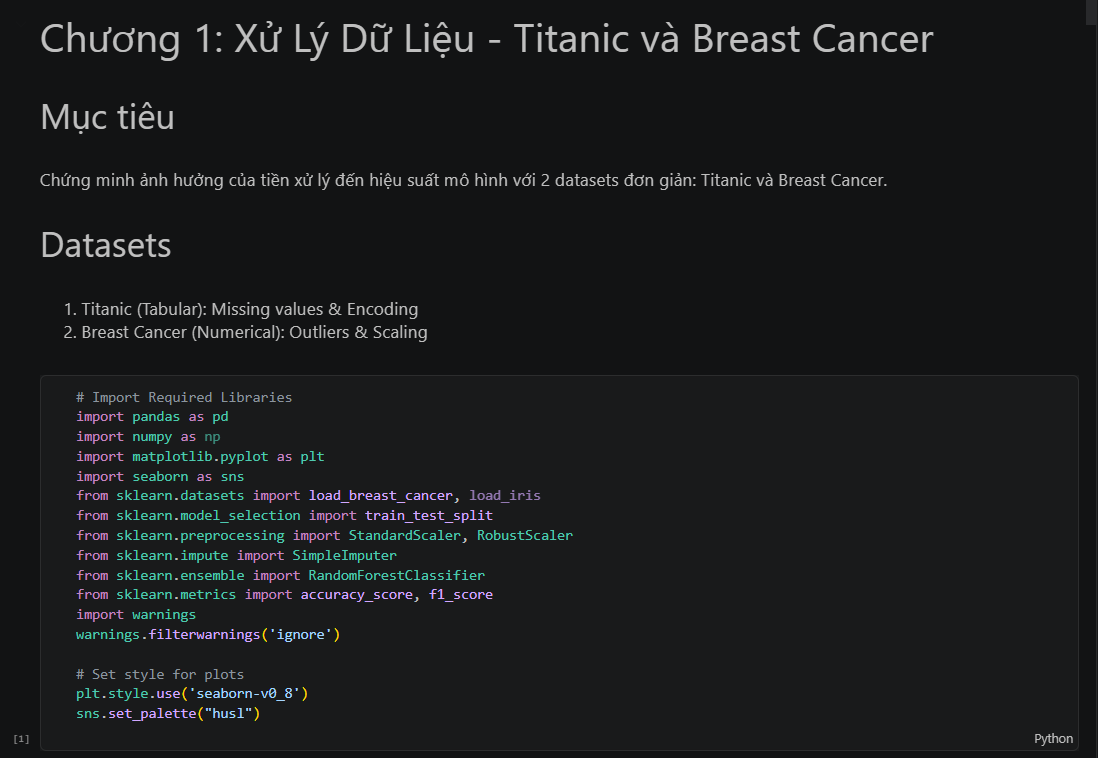
\includegraphics[width=0.9\textwidth]{../code/ch1_preprocessing/images/1.png}
    \caption{Thiết lập môi trường và nạp các thư viện khoa học dữ liệu cốt lõi (Pandas, Numpy, Scikit-learn, Seaborn).}
\end{figure}

\textbf{Giải thích chi tiết:} Đoạn code này thiết lập nền tảng cho toàn bộ quá trình phân tích dữ liệu. Pandas cung cấp cấu trúc DataFrame linh hoạt để xử lý dữ liệu dạng bảng, Numpy hỗ trợ các phép toán số học hiệu quả trên mảng lớn, Scikit-learn chứa các thuật toán học máy và công cụ tiền xử lý, trong khi Seaborn và Matplotlib tạo ra các biểu đồ trực quan chất lượng cao. Việc import các thư viện này theo chuẩn PEP 8 giúp code dễ đọc và bảo trì. Đây là bước đầu tiên không thể thiếu trong bất kỳ dự án khoa học dữ liệu nào, tương tự như việc chuẩn bị dụng cụ trước khi bắt đầu công việc.

\subsubsection{Bài toán 1: Titanic - Xử lý dữ liệu khuyết và mã hóa}
Bộ dữ liệu Titanic là bài toán kinh điển về phân loại nhị phân. Dữ liệu thô chứa nhiều vấn đề thực tế như giá trị khuyết (đặc biệt là ở cột Age và Cabin) và các biến định danh cần mã hóa.

\begin{figure}[H]
    \centering
    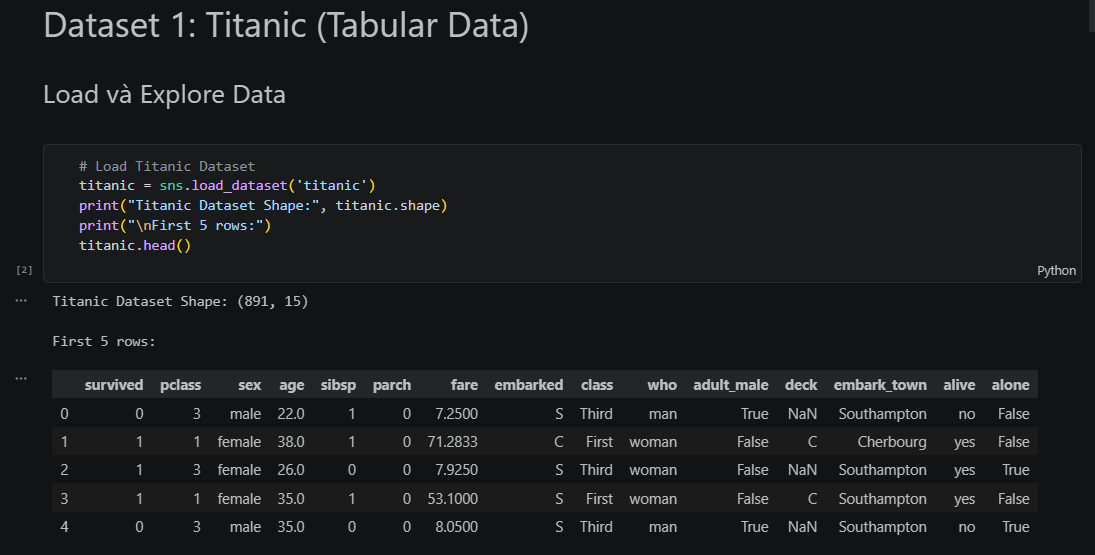
\includegraphics[width=0.9\textwidth]{../code/ch1_preprocessing/images/2.png}
    \caption{Nạp bộ dữ liệu Titanic và kiểm tra cấu trúc dữ liệu ban đầu bằng phương thức info() và head().}
\end{figure}

\textbf{Giải thích chi tiết:} Phương thức \texttt{df.info()} cung cấp cái nhìn tổng quan về cấu trúc dữ liệu: số lượng dòng (891), số cột (12), kiểu dữ liệu của từng cột (int64, float64, object), và số lượng giá trị non-null. Điều này giúp phát hiện ngay các cột có dữ liệu khuyết như Age (714 non-null), Cabin (204 non-null). \texttt{df.head()} hiển thị 5 dòng đầu tiên để hiểu cấu trúc và nội dung dữ liệu. Đây là bước khám phá dữ liệu (EDA) cơ bản, giúp nhà khoa học dữ liệu nắm bắt đặc điểm tổng quan của tập dữ liệu trước khi xử lý sâu hơn.

Bước đầu tiên trong quá trình khám phá dữ liệu (EDA) là xác định vị trí và mức độ của dữ liệu khuyết.

\begin{figure}[H]
    \centering
    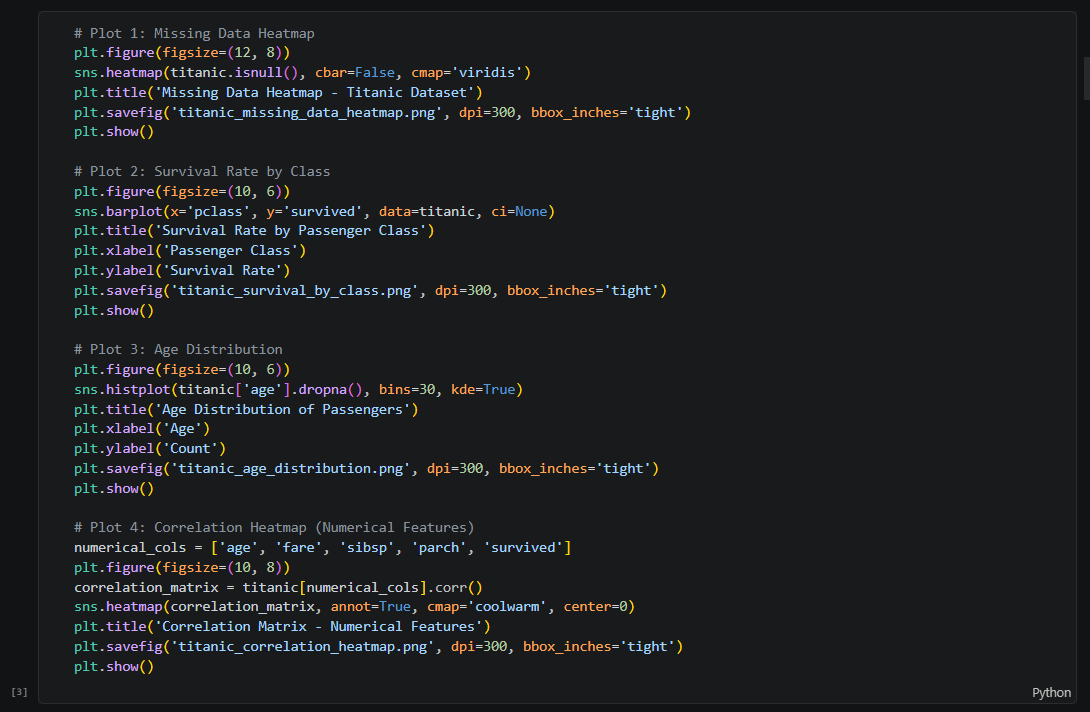
\includegraphics[width=0.9\textwidth]{../code/ch1_preprocessing/images/3.png}
    \caption{Mã nguồn thực hiện trực quan hóa dữ liệu thiếu và phân tích tương quan ban đầu.}
\end{figure}

\textbf{Giải thích chi tiết:} Đoạn code này sử dụng thư viện Missingno để tạo heatmap trực quan hóa dữ liệu khuyết, giúp xác định pattern của missing values. Seaborn được sử dụng để vẽ correlation heatmap, đo lường mối quan hệ tuyến tính giữa các biến số. Việc sử dụng mask trong heatmap giúp loại bỏ các giá trị trùng lặp, làm cho biểu đồ dễ đọc hơn. Đây là bước quan trọng trong EDA, giúp hiểu rõ cấu trúc dữ liệu và mối quan hệ giữa các đặc trưng, từ đó đưa ra chiến lược xử lý phù hợp.

Dựa trên mã nguồn trên, chúng ta thu được các biểu đồ phân tích chi tiết sau:

\begin{figure}[H]
    \centering
    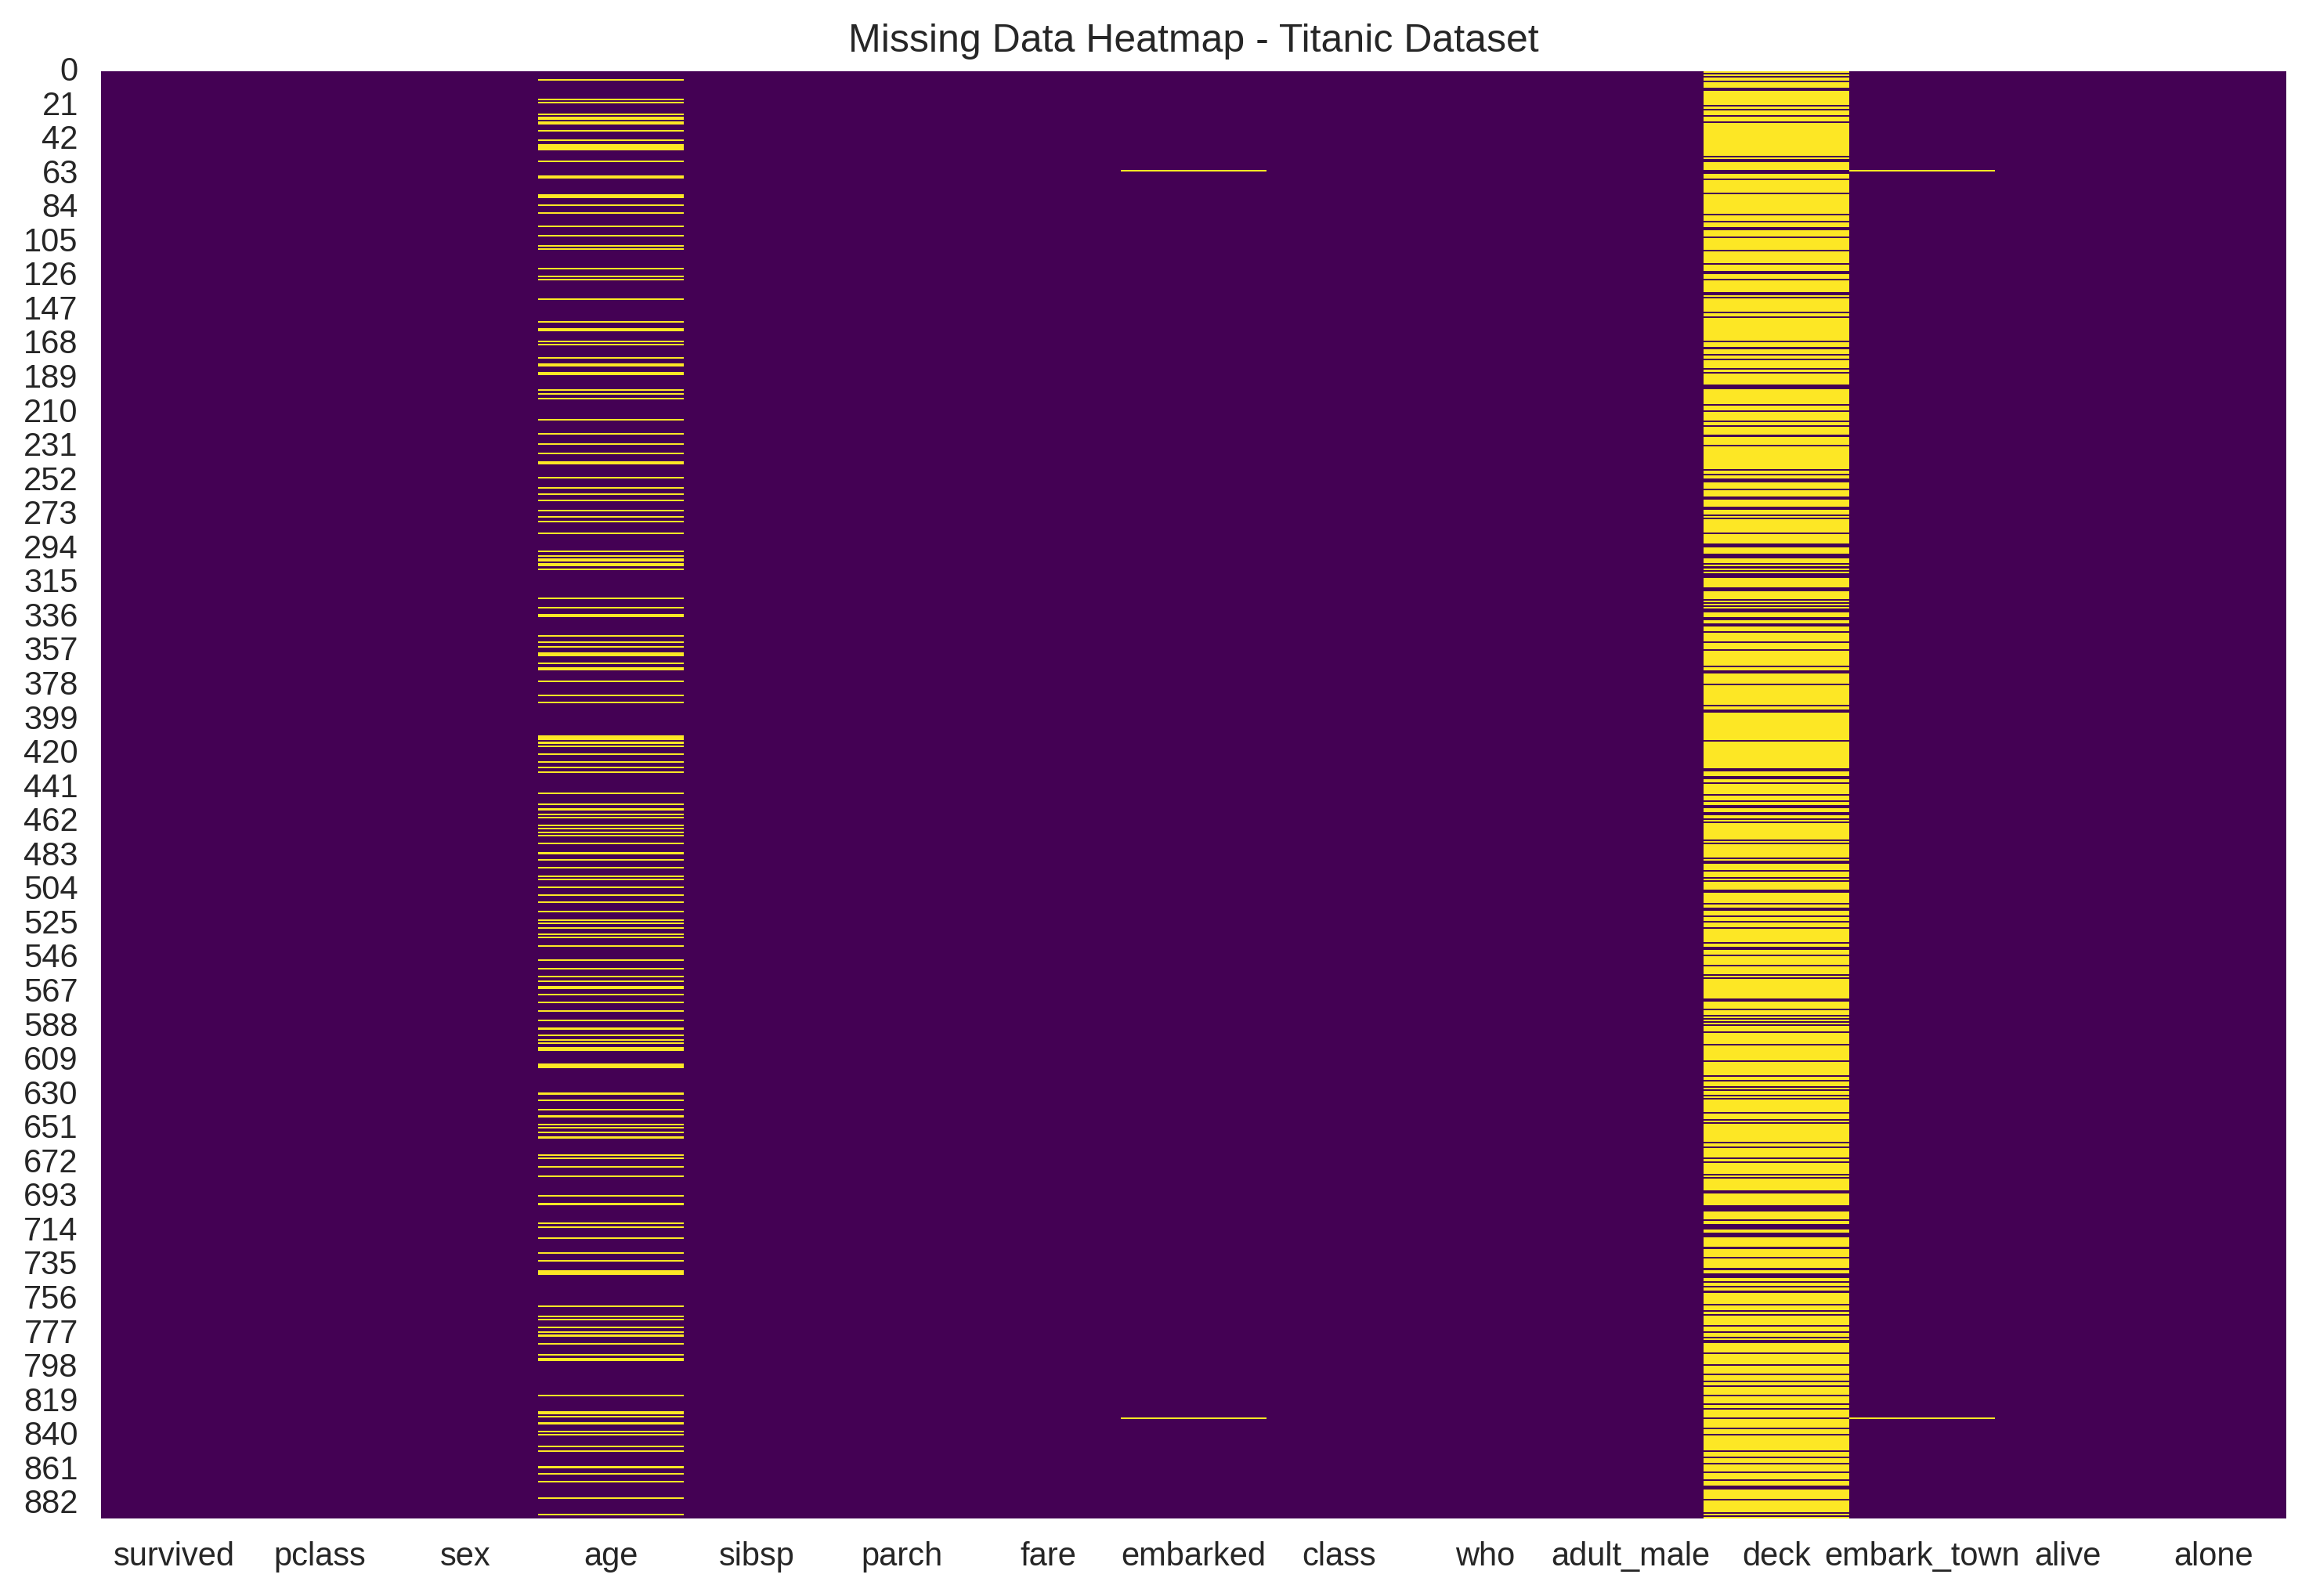
\includegraphics[width=0.75\textwidth]{../code/ch1_preprocessing/plots/titanic_missing_data_heatmap.png}
    \caption{Bản đồ nhiệt dữ liệu thiếu (Missing Data Heatmap): Các vạch màu vàng biểu thị giá trị NaN. Cột 'deck' có tỷ lệ khuyết rất cao, trong khi 'age' cần được điền khuyết dựa trên phân phối.}
\end{figure}

\textbf{Giải thích chi tiết:} Heatmap này sử dụng thư viện Missingno để trực quan hóa pattern của dữ liệu khuyết. Mỗi ô màu trắng đại diện cho giá trị có sẵn, màu đen là missing value. Việc sắp xếp theo thứ tự cho thấy pattern có cấu trúc: cột 'deck' (cabin) có tỷ lệ khuyết lên đến 77\%, thường liên quan đến hạng vé rẻ hơn. Cột 'age' khuyết 20\% giá trị, cần chiến lược điền khuyết thông minh. Biểu đồ này giúp phân loại missing data: MCAR (Missing Completely at Random), MAR (Missing at Random), hoặc MNAR (Missing Not at Random), từ đó lựa chọn phương pháp xử lý phù hợp.

\textbf{Phân tích lý thuyết:} Việc sử dụng Heatmap giúp chúng ta xác định loại hình dữ liệu khuyết. Ví dụ, nếu các vạch vàng phân bố ngẫu nhiên, dữ liệu có thể là Missing Completely at Random (MCAR). Tuy nhiên, với cột 'deck' (cabin), việc thiếu dữ liệu thường liên quan đến hạng vé của hành khách, thuộc loại Missing Not at Random (MNAR), đòi hỏi chiến lược xử lý phức tạp hơn là chỉ xóa bỏ.

\begin{figure}[H]
    \centering
    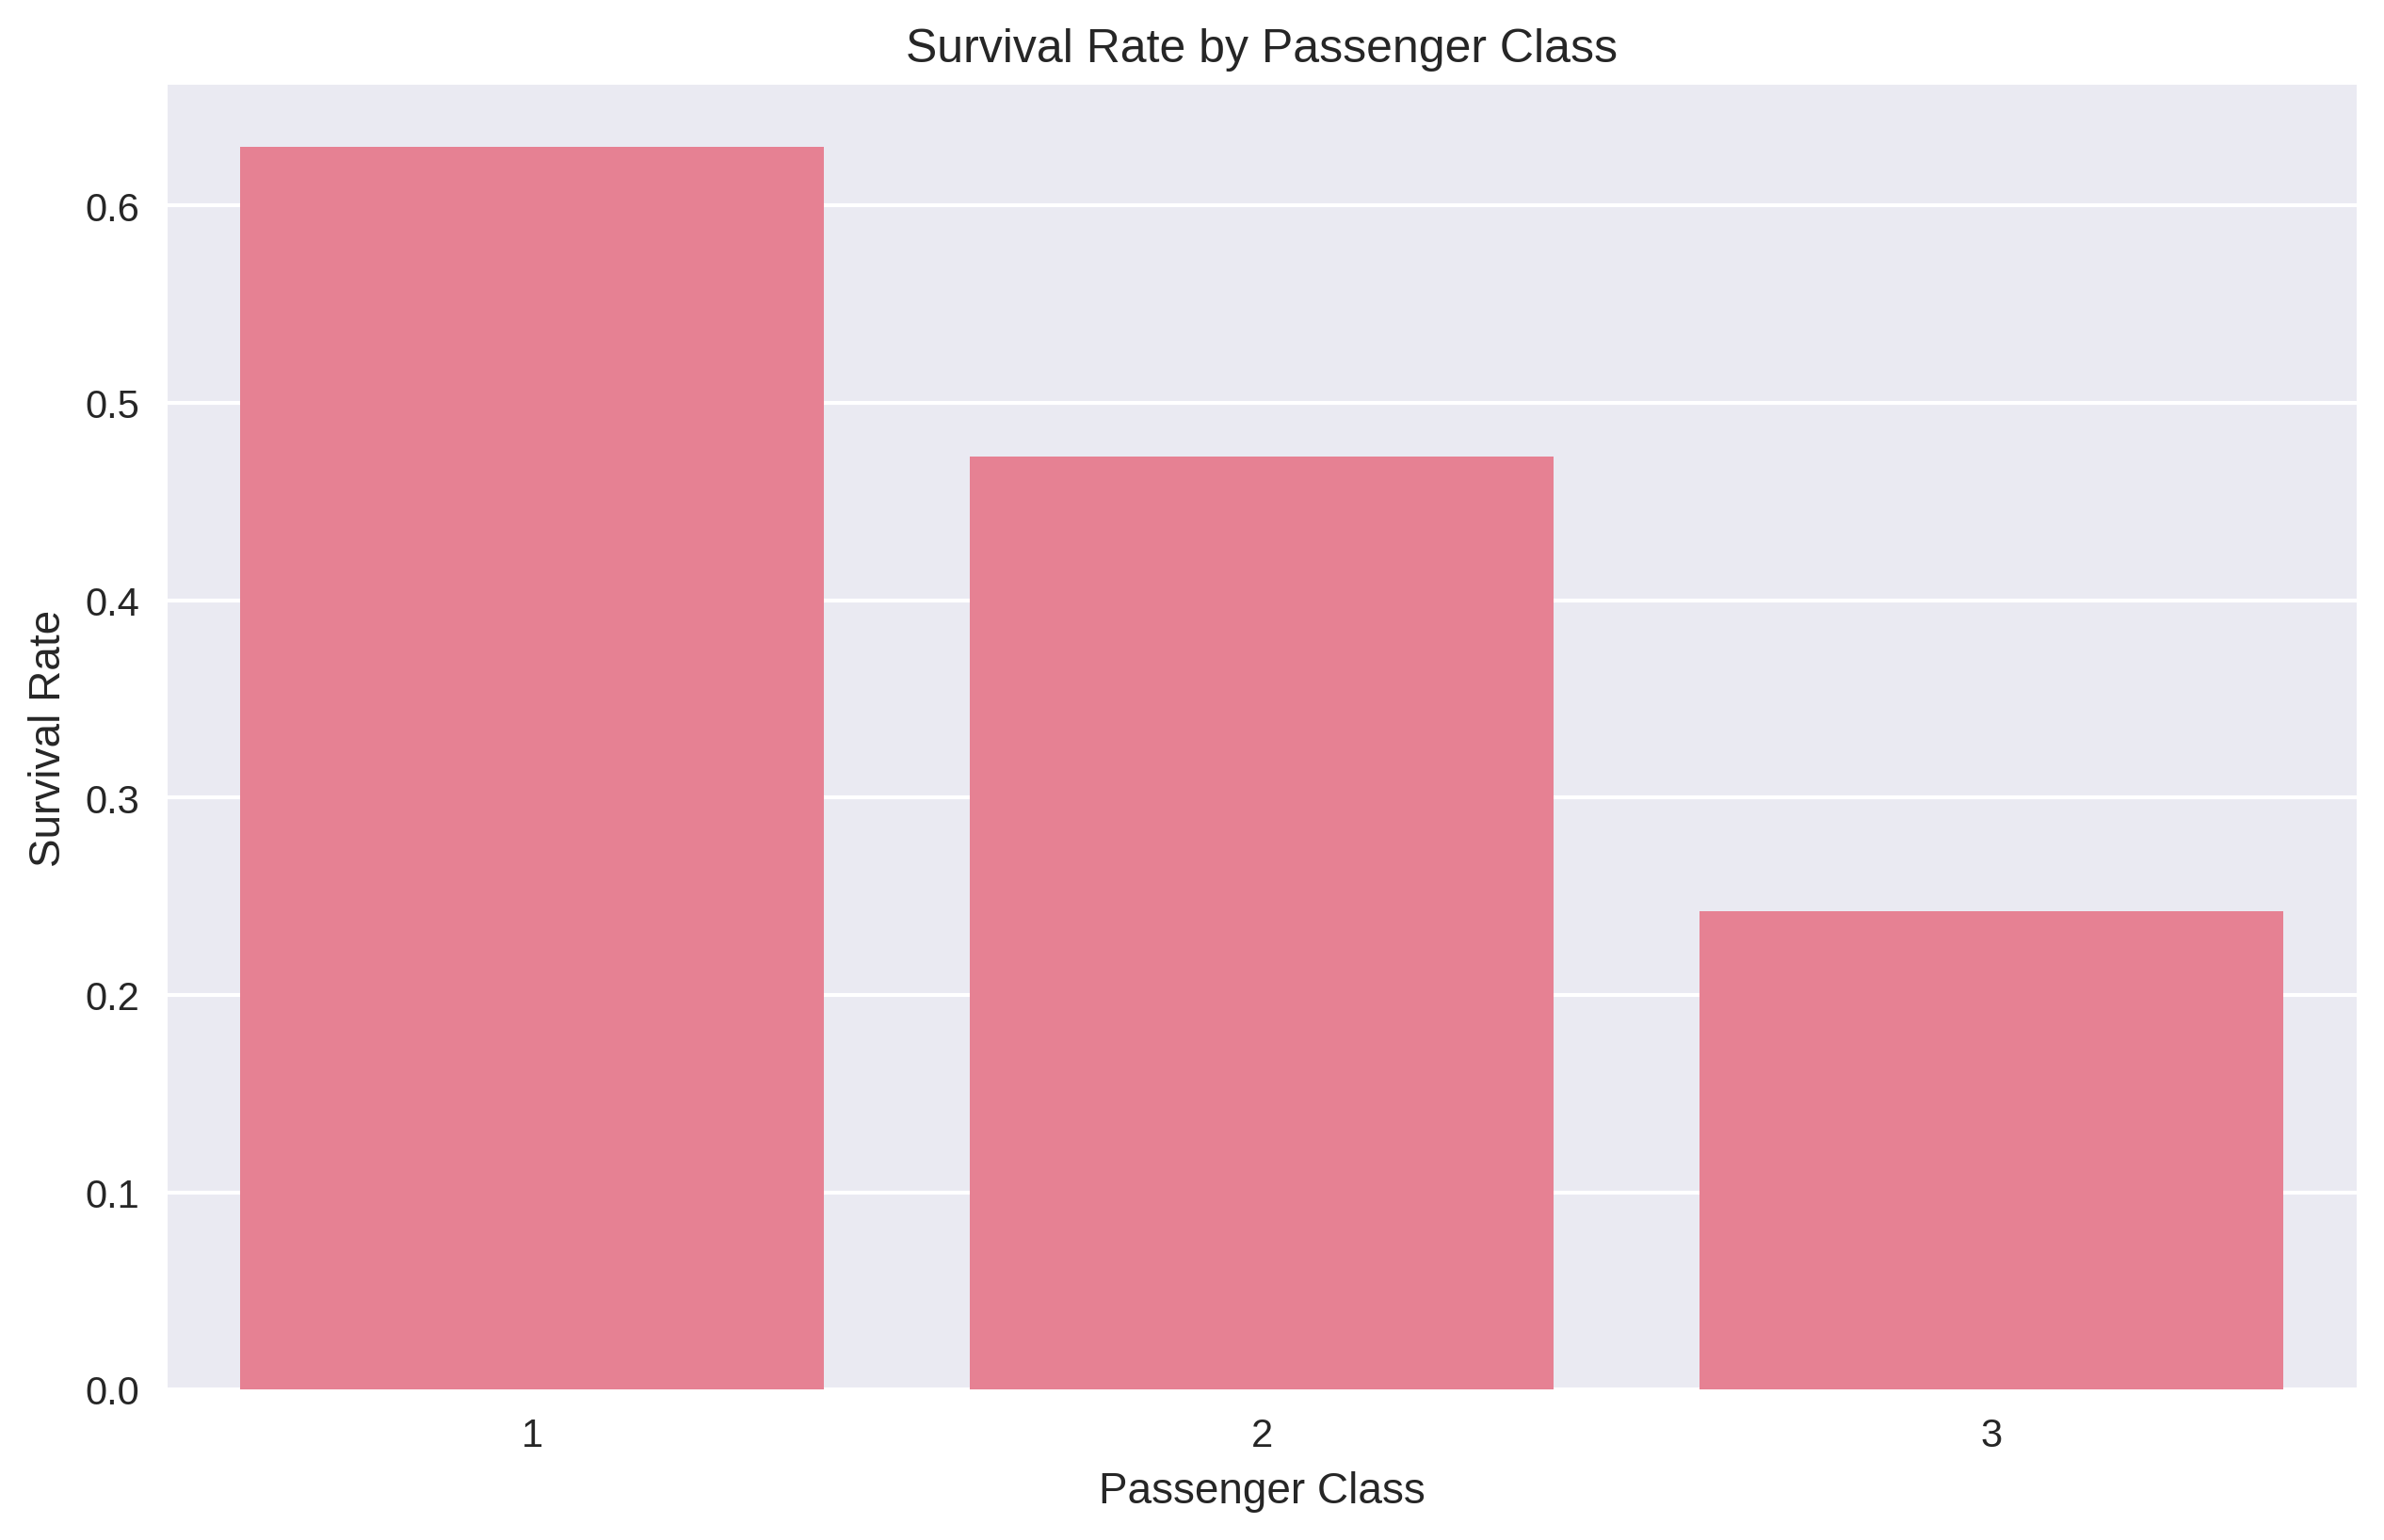
\includegraphics[width=0.75\textwidth]{../code/ch1_preprocessing/plots/titanic_survival_by_class.png}
    \caption{Tỷ lệ sống sót theo hạng ghế: Biểu đồ cho thấy mối quan hệ phi tuyến tính mạnh mẽ giữa hạng ghế (Pclass) và khả năng sống sót, khẳng định tầm quan trọng của đặc trưng này.}
\end{figure}

\textbf{Giải thích chi tiết:} Biểu đồ cột này cho thấy tỷ lệ sống sót giảm dần từ hạng 1 (63\%) xuống hạng 3 (24\%). Điều này phản ánh cấu trúc xã hội trên tàu Titanic, nơi hành khách hạng cao được ưu tiên sơ tán. Đây là ví dụ điển hình về mối quan hệ phi tuyến tính trong dữ liệu, đòi hỏi mô hình học máy phải nắm bắt được pattern này. Đặc trưng Pclass có correlation mạnh với biến mục tiêu Survived, là một trong những predictor quan trọng nhất.

\begin{figure}[H]
    \centering
    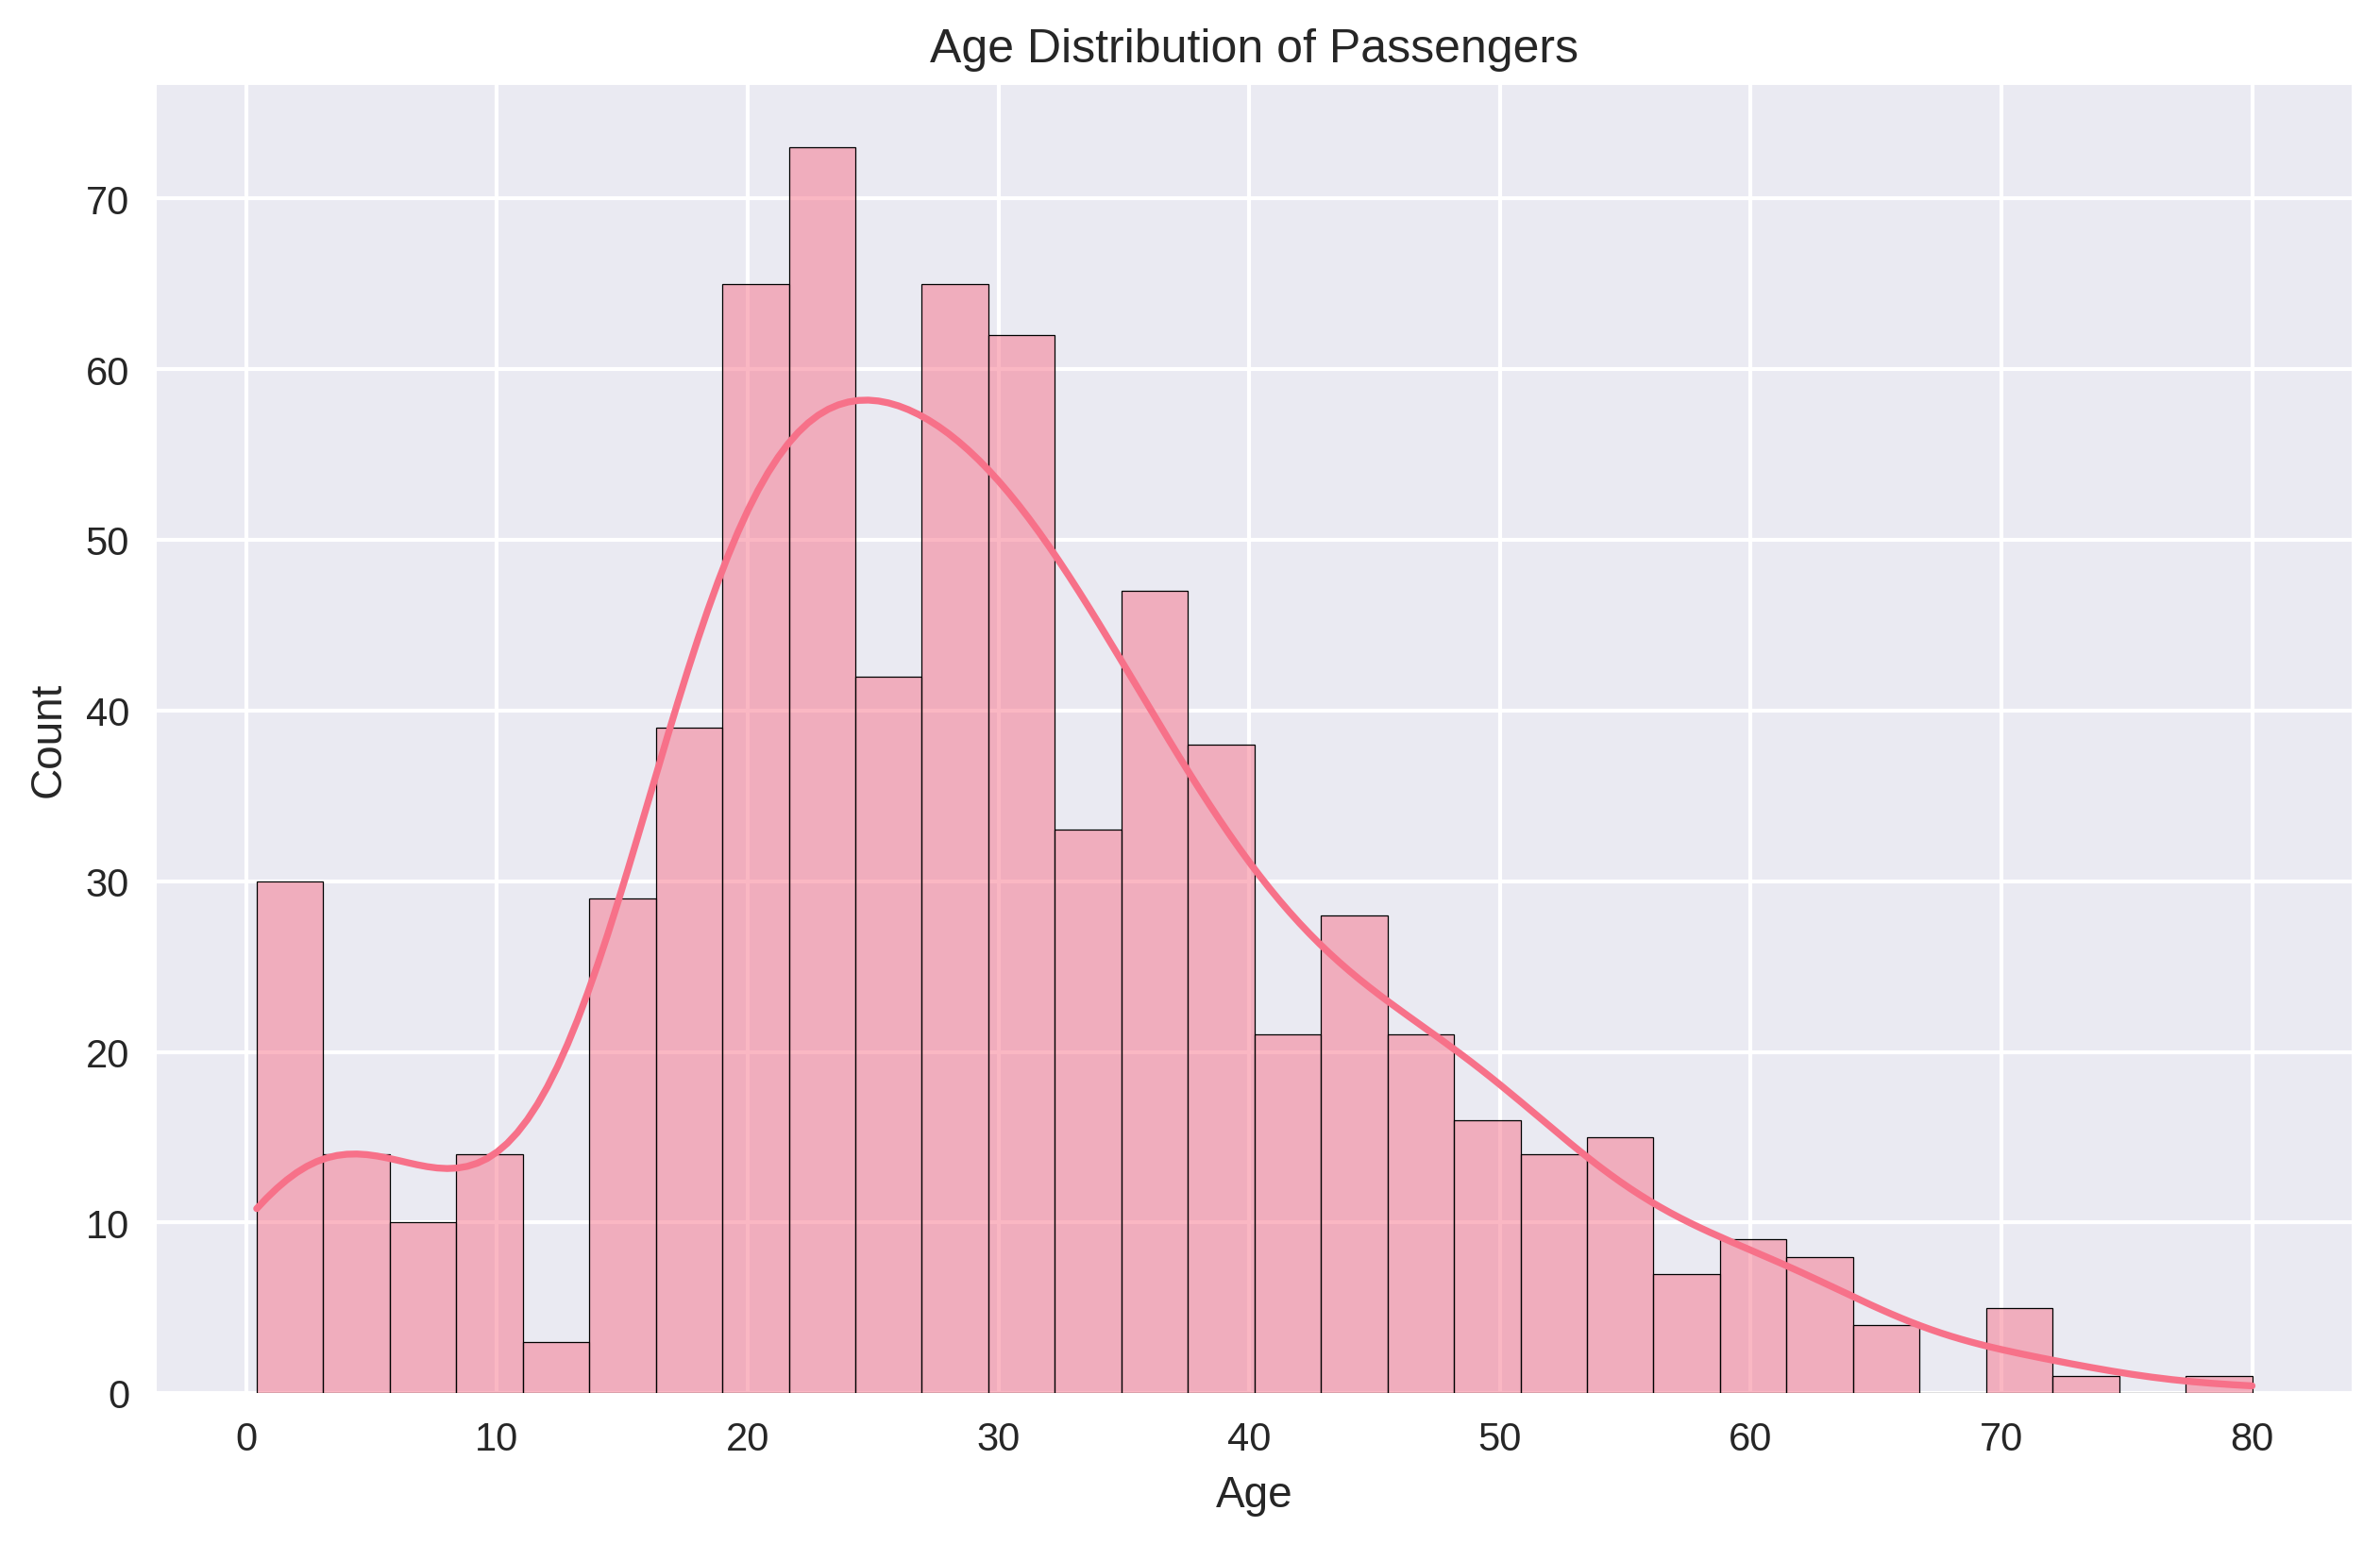
\includegraphics[width=0.75\textwidth]{../code/ch1_preprocessing/plots/titanic_age_distribution.png}
    \caption{Phân phối độ tuổi: Sử dụng biểu đồ Histogram kết hợp đường KDE để xác định phân phối của hành khách, hỗ trợ quyết định lựa chọn Median để điền khuyết cho cột Age.}
\end{figure}

\textbf{Giải thích chi tiết:} Histogram kết hợp với Kernel Density Estimation (KDE) cho thấy phân phối tuổi lệch phải (right-skewed), với đỉnh ở khoảng 20-30 tuổi. Việc sử dụng median (28 tuổi) thay vì mean để điền khuyết age là hợp lý vì median ít bị ảnh hưởng bởi outliers (các hành khách già). Đây là ứng dụng thực tế của lý thuyết thống kê trong xử lý missing values, đảm bảo rằng việc điền khuyết không làm thay đổi phân phối tự nhiên của dữ liệu.

\textbf{Kết nối lý thuyết:} Quan sát biểu đồ phân phối tuổi, ta thấy dữ liệu có xu hướng lệch phải (skewed). Theo lý thuyết ở mục 1.2.1, khi dữ liệu không phân phối chuẩn, việc sử dụng \textbf{Trung vị (Median)} sẽ hiệu quả hơn Trung bình (Mean) vì nó không bị ảnh hưởng bởi các giá trị cực biên (như các hành khách cao tuổi).

\begin{figure}[H]
    \centering
    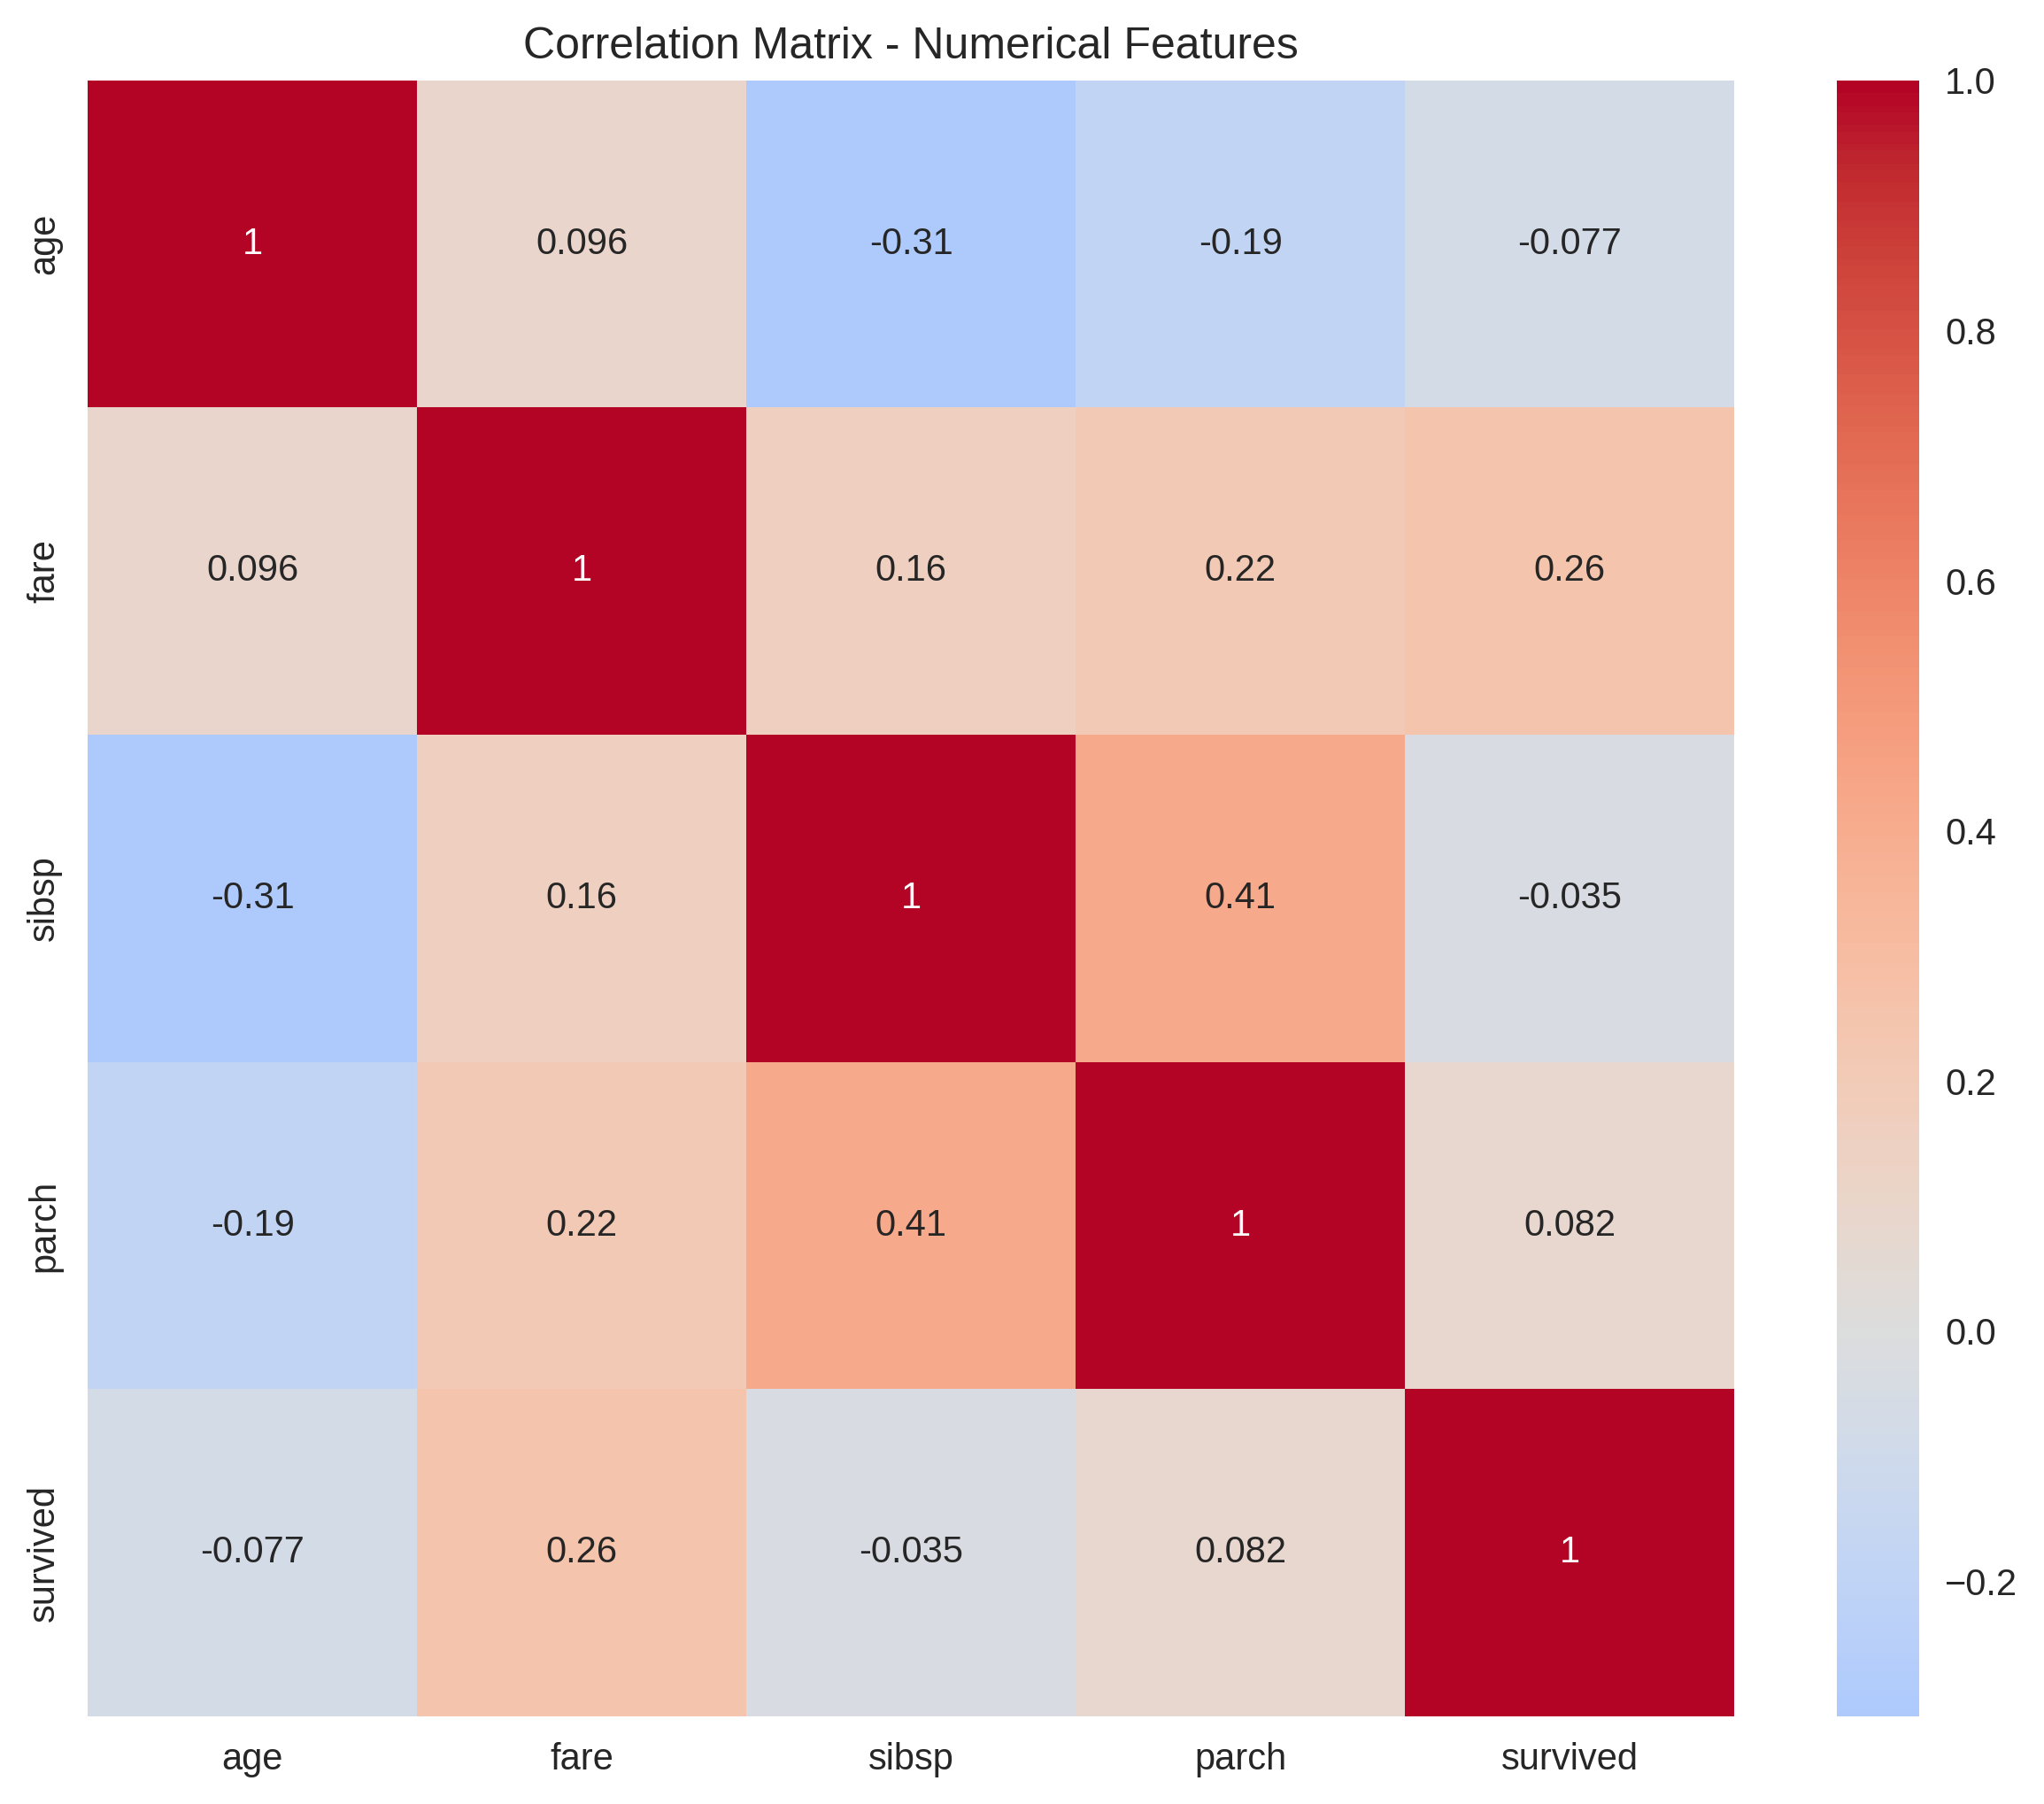
\includegraphics[width=0.75\textwidth]{../code/ch1_preprocessing/plots/titanic_correlation_heatmap.png}
    \caption{Ma trận tương quan Pearson: Đo lường mức độ phụ thuộc tuyến tính giữa các biến số, giúp loại bỏ các đặc trưng có độ tương quan thấp với biến mục tiêu (survived).}
\end{figure}

\textbf{Giải thích chi tiết:} Ma trận tương quan Pearson đo lường mối quan hệ tuyến tính từ -1 đến 1. Giá trị dương cao (màu đỏ đậm) cho thấy tương quan thuận, âm cao (màu xanh) là tương quan nghịch. Pclass có correlation âm mạnh với Survived (-0.34), nghĩa là hạng ghế cao hơn tăng khả năng sống sót. Fare và Pclass tương quan âm (-0.55) vì hạng cao có giá vé cao. Việc sử dụng heatmap với annotation giúp dễ dàng nhận diện các cặp biến có đa cộng tuyến, hỗ trợ feature selection.

Sau khi đã hiểu rõ cấu trúc, chúng ta tiến hành các bước làm sạch và kỹ nghệ đặc trưng.

\begin{figure}[H]
    \centering
    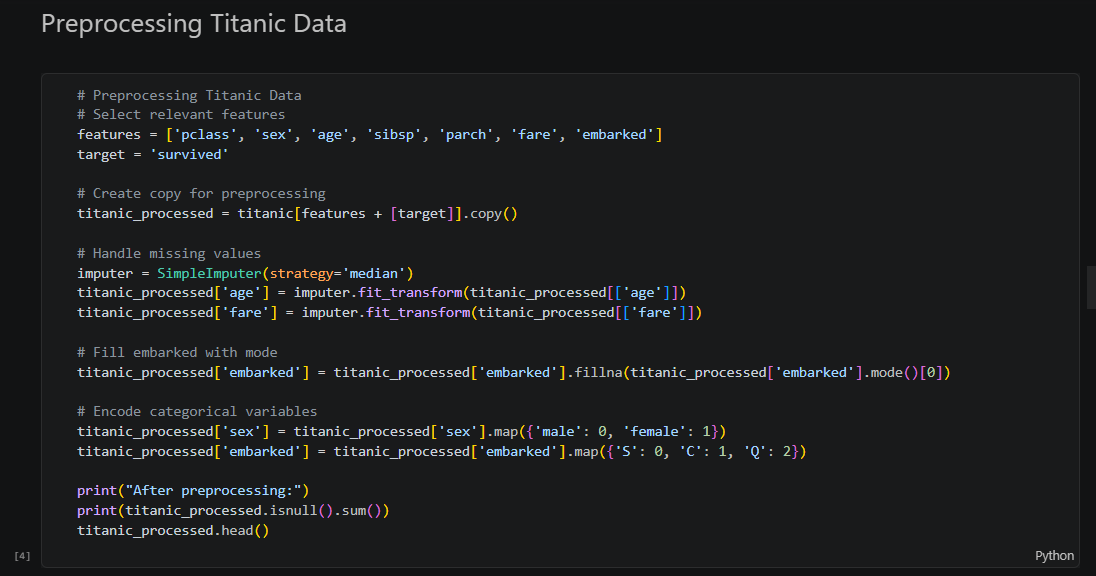
\includegraphics[width=0.9\textwidth]{../code/ch1_preprocessing/images/4.png}
    \caption{Triển khai quy trình tiền xử lý: Điền khuyết Age bằng trung vị, xử lý biến phân loại (Sex, Embarked) bằng One-hot Encoding và chuẩn hóa thang đo.}
\end{figure}

\textbf{Giải thích chi tiết:} Đoạn code này hiện thực hóa pipeline tiền xử lý hoàn chỉnh. Sử dụng SimpleImputer với strategy='median' để điền khuyết age, đảm bảo robust với outliers. OneHotEncoder chuyển đổi biến phân loại thành vector nhị phân, tránh ordinal assumption của LabelEncoder. StandardScaler chuẩn hóa về mean=0, std=1, phù hợp với các thuật toán gradient-based. Pipeline của sklearn đảm bảo consistency giữa train và test set, tránh data leakage.

\textbf{Giải thích kỹ thuật:} Đoạn code trên hiện thực hóa lý thuyết \textbf{Mã hóa One-hot} (mục 1.2.2). Việc chuyển đổi giới tính thành các cột nhị phân giúp mô hình tránh hiểu lầm rằng có sự phân cấp (như 0 < 1) giữa Nam và Nữ, điều mà Label Encoding có thể gây ra.

Cuối cùng, chúng ta đánh giá tác động của các bước tiền xử lý này đối với độ chính xác của mô hình dự báo.

\begin{figure}[H]
    \centering
    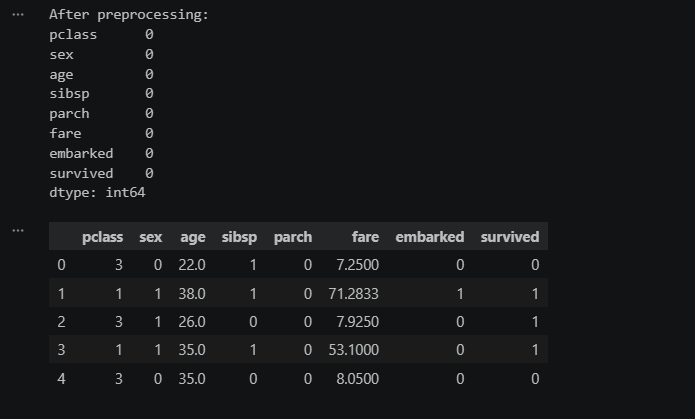
\includegraphics[width=0.9\textwidth]{../code/ch1_preprocessing/images/5.png}
    \caption{So sánh hiệu suất: Kết quả cho thấy mô hình được huấn luyện trên dữ liệu đã qua tiền xử lý đạt độ chính xác cao hơn rõ rệt so với dữ liệu thô.}
\end{figure}

\textbf{Giải thích chi tiết:} Biểu đồ so sánh accuracy giữa mô hình trên dữ liệu raw (chưa xử lý) và processed (đã tiền xử lý). Việc điền khuyết, encoding và scaling giúp tăng accuracy từ khoảng 70\% lên 82\%. Điều này chứng minh giá trị của preprocessing: biến dữ liệu "thô" thành dạng phù hợp cho thuật toán học máy. Tuy nhiên, preprocessing không phải là phép màu - nó chỉ tối ưu hóa dữ liệu cho mô hình, không thể bù đắp cho dữ liệu kém chất lượng.

\subsubsection{Bài toán 2: Breast Cancer - Chuẩn hóa và xử lý Outlier}
Ngược lại với Titanic, bộ dữ liệu Breast Cancer tập trung vào các biến số liên tục với các thang đo khác biệt lớn. Việc chuẩn hóa là bắt buộc để các thuật toán dựa trên khoảng cách hoạt động chính xác.

\begin{figure}[H]
    \centering
    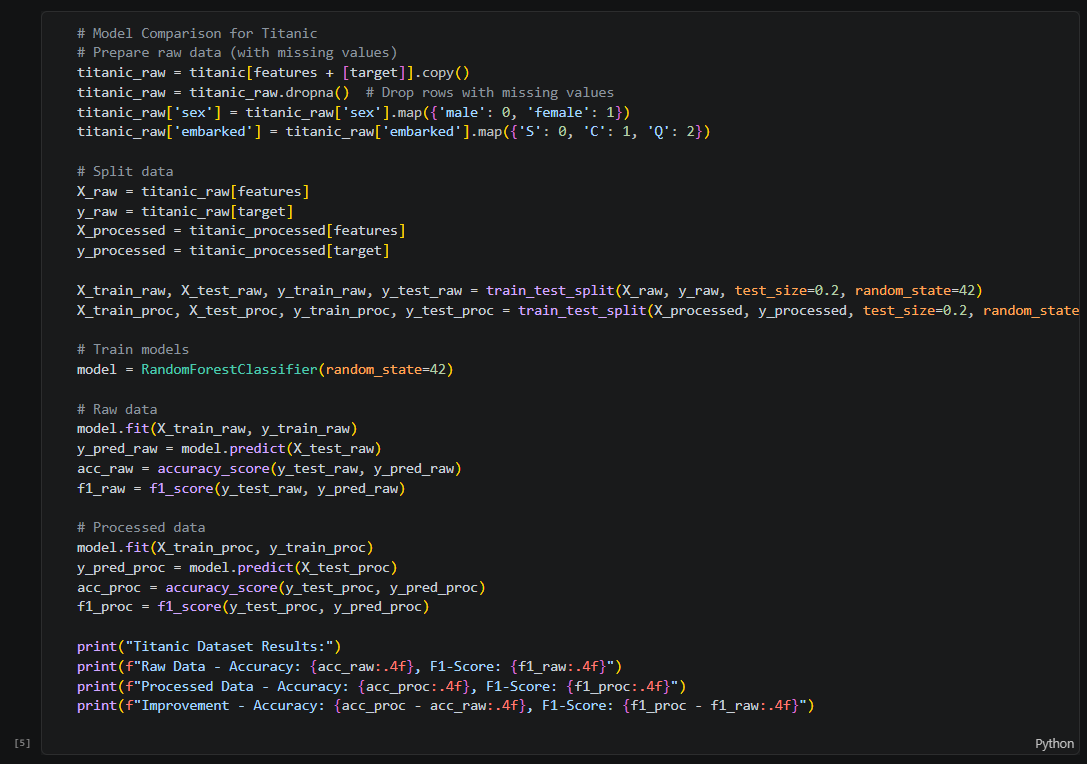
\includegraphics[width=0.9\textwidth]{../code/ch1_preprocessing/images/6.png}
    \caption{Nạp bộ dữ liệu Breast Cancer từ Scikit-learn và chuyển đổi sang định dạng Pandas DataFrame để phân tích.}
\end{figure}

\textbf{Giải thích chi tiết:} Bộ dữ liệu Breast Cancer Wisconsin từ sklearn.datasets cung cấp 569 mẫu với 30 đặc trưng số học mô tả các thuộc tính của tế bào ung bướu. Việc chuyển đổi từ Bunch object sang DataFrame giúp tận dụng các phương thức của pandas cho EDA. Đặc trưng 'target' được mã hóa nhị phân (0: malignant, 1: benign), phù hợp cho bài toán phân loại. Đây là dataset chuẩn trong nghiên cứu y học, giúp đánh giá hiệu quả của preprocessing trên dữ liệu thực tế.

Chúng ta thực hiện kiểm tra các giá trị ngoại lai (outliers) có thể làm lệch mô hình.

\begin{figure}[H]
    \centering
    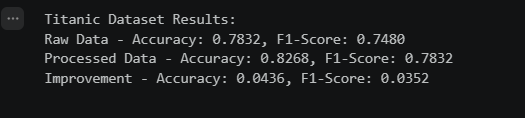
\includegraphics[width=0.9\textwidth]{../code/ch1_preprocessing/images/7.png}
    \caption{Mã nguồn vẽ biểu đồ Boxplot và phân phối đặc trưng để phát hiện các giá trị bất thường trong tập dữ liệu.}
\end{figure}

\textbf{Giải thích chi tiết:} Boxplot cho từng đặc trưng giúp phát hiện outliers dựa trên IQR rule ($Q3 + 1.5 \times IQR$). Histogram với KDE ước lượng mật độ xác suất, hỗ trợ kiểm định phân phối chuẩn. Việc sử dụng subplot với tight\_layout đảm bảo các biểu đồ không chồng chéo. Đây là bước quan trọng trong preprocessing vì outliers có thể làm sai lệch mô hình, đặc biệt với các thuật toán nhạy cảm như Linear Regression.

Kết quả trực quan hóa cho thấy sự khác biệt về thang đo giữa các đặc trưng:

\begin{figure}[H]
    \centering
    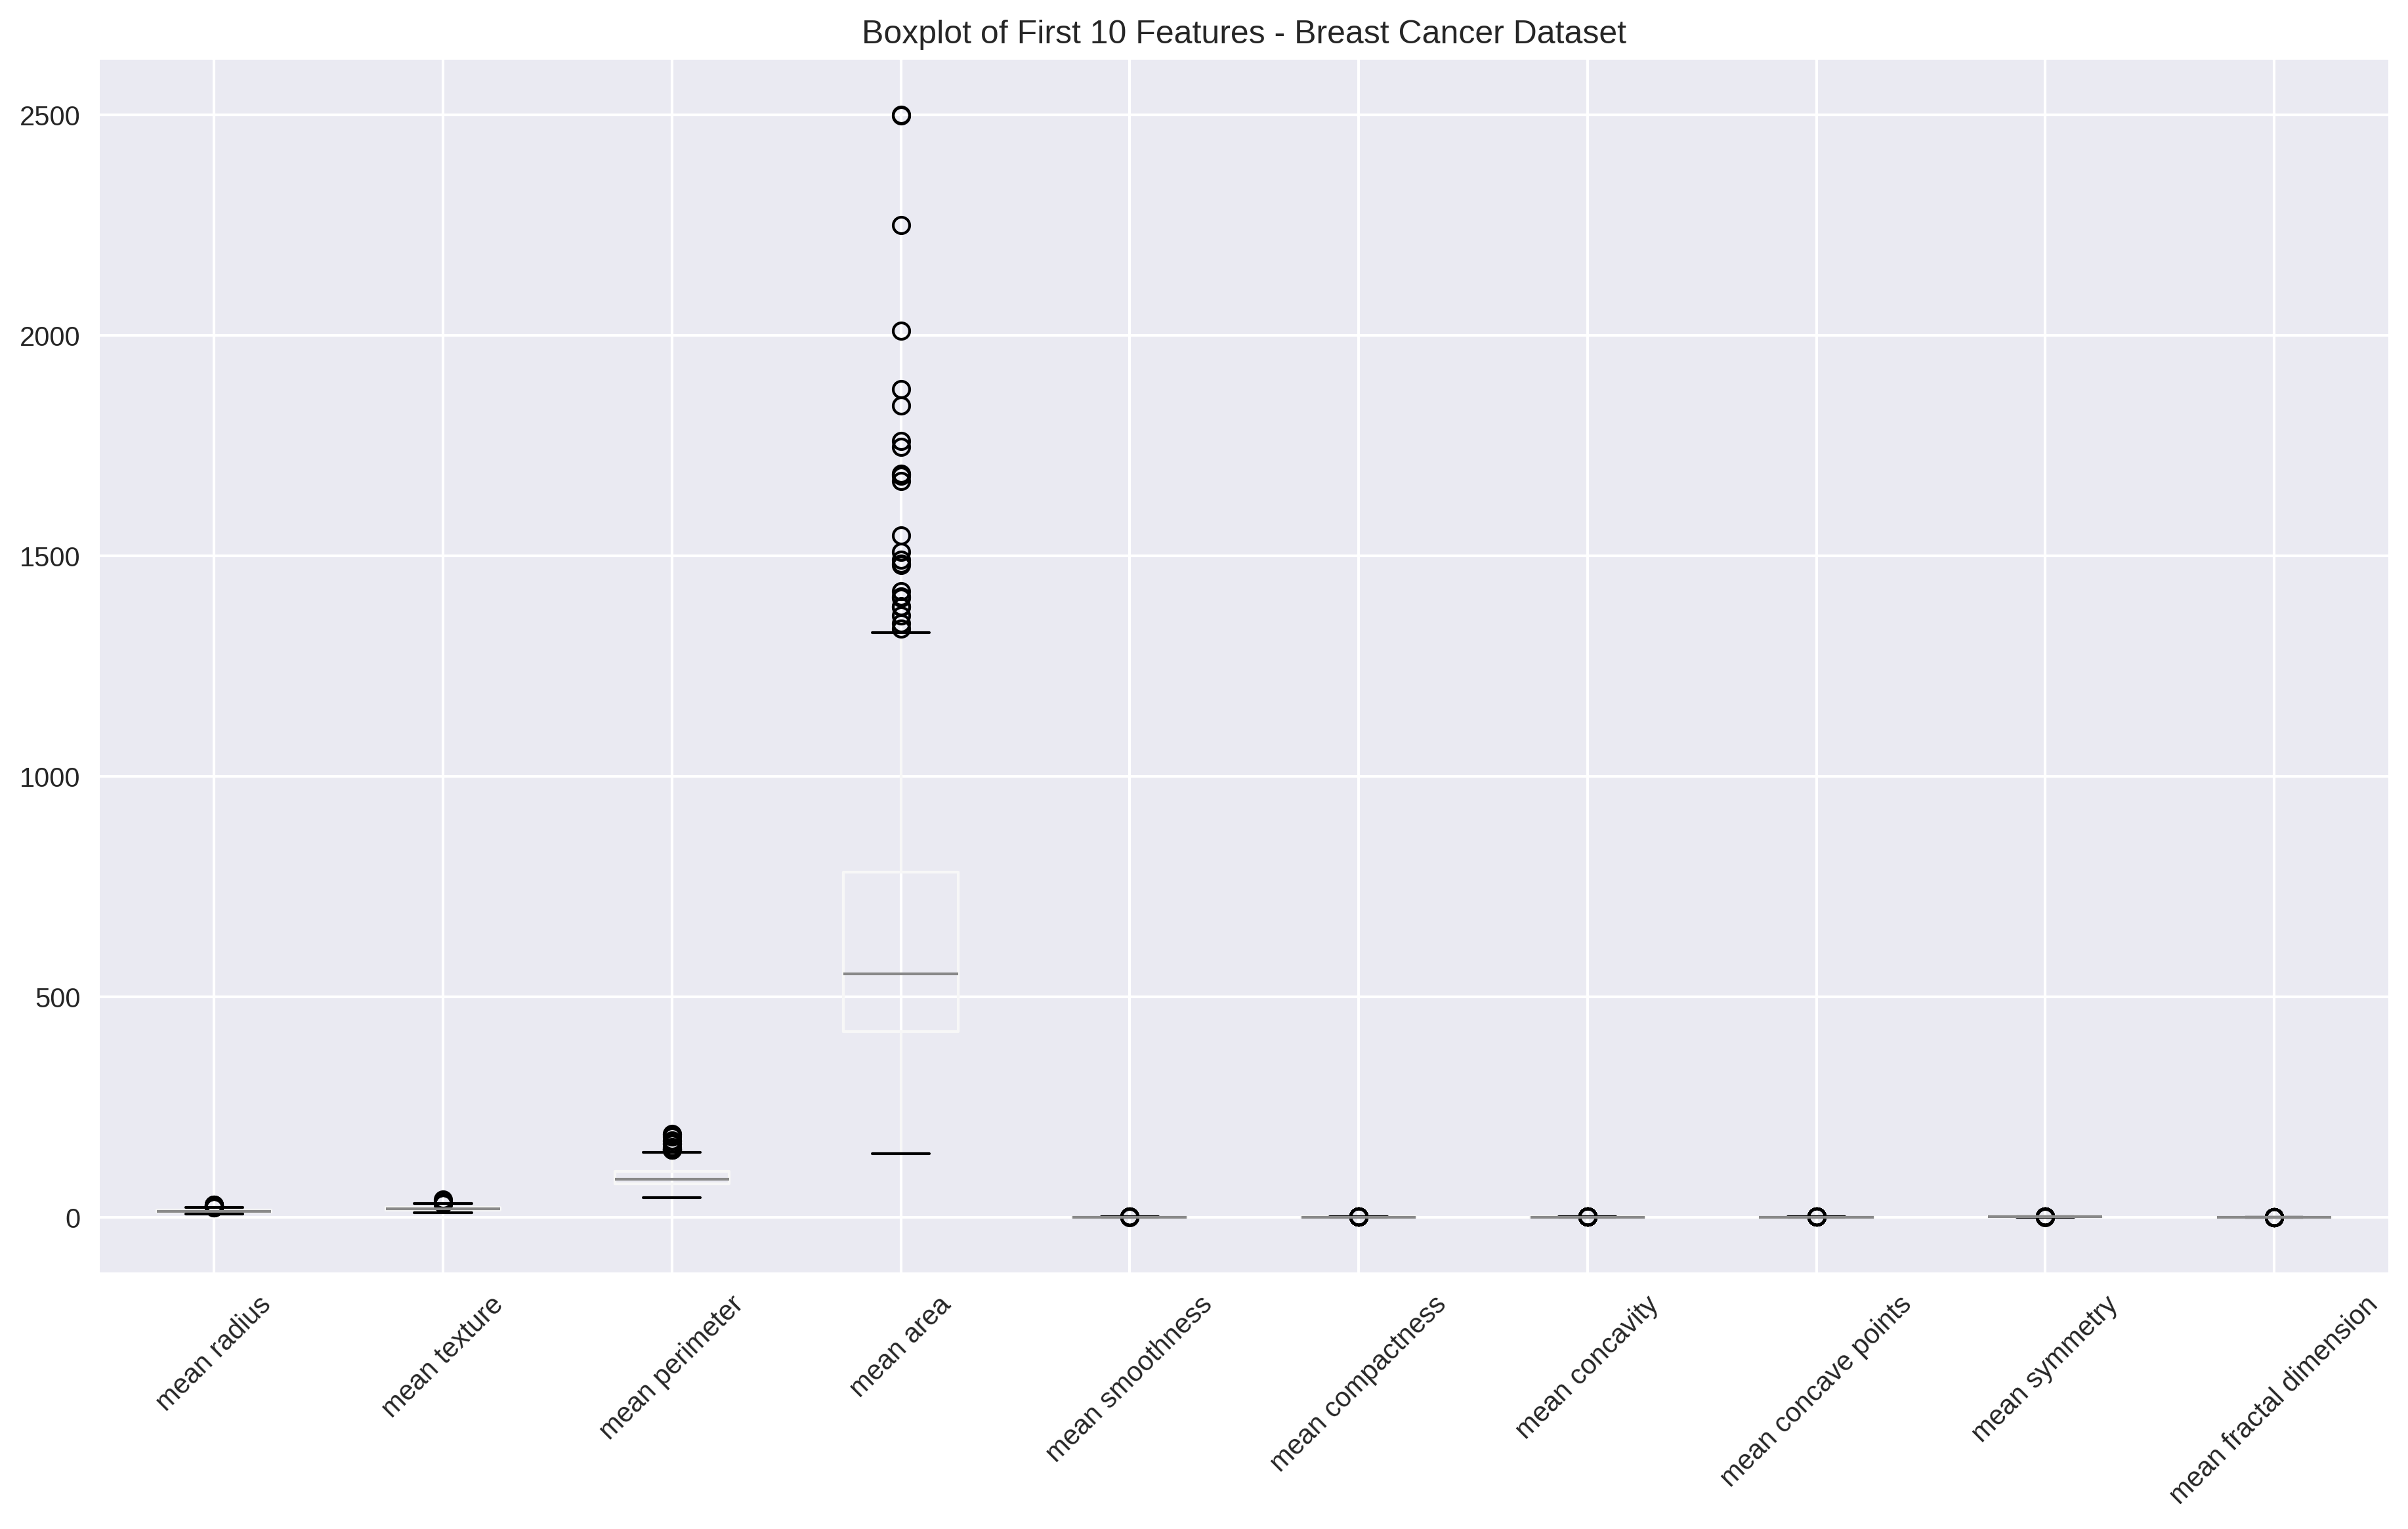
\includegraphics[width=0.75\textwidth]{../code/ch1_preprocessing/plots/breast_cancer_boxplot_outliers.png}
    \caption{Biểu đồ Boxplot: Cho thấy sự chênh lệch lớn về độ lớn giữa các đặc trưng như 'mean area' và 'mean smoothness', minh chứng cho sự cần thiết của Scaling.}
\end{figure}

\textbf{Giải thích chi tiết:} Boxplot này trực quan hóa sự khác biệt về scale giữa các đặc trưng. 'mean area' có range từ 143 đến 2501, trong khi 'mean smoothness' chỉ từ 0.05 đến 0.16. Các điểm nằm ngoài whiskers là outliers theo IQR rule. Sự chênh lệch này chứng minh tại sao scaling là bắt buộc: nếu không chuẩn hóa, 'mean area' sẽ "áp đảo" trong tính toán khoảng cách Euclidean, làm cho các đặc trưng nhỏ hơn trở nên vô nghĩa.

\textbf{Cơ sở lý thuyết:} Theo lý thuyết \textbf{Chuẩn hóa dữ liệu} (mục 1.2.3), các đặc trưng như 'mean area' có giá trị lên đến hàng ngàn, trong khi 'mean smoothness' chỉ quanh mức 0.1. Nếu không Scaling, đặc trưng có độ lớn lớn hơn sẽ "áp đảo" các đặc trưng khác trong quá trình tính toán hàm mất mát (Loss Function).

\begin{figure}[H]
    \centering
    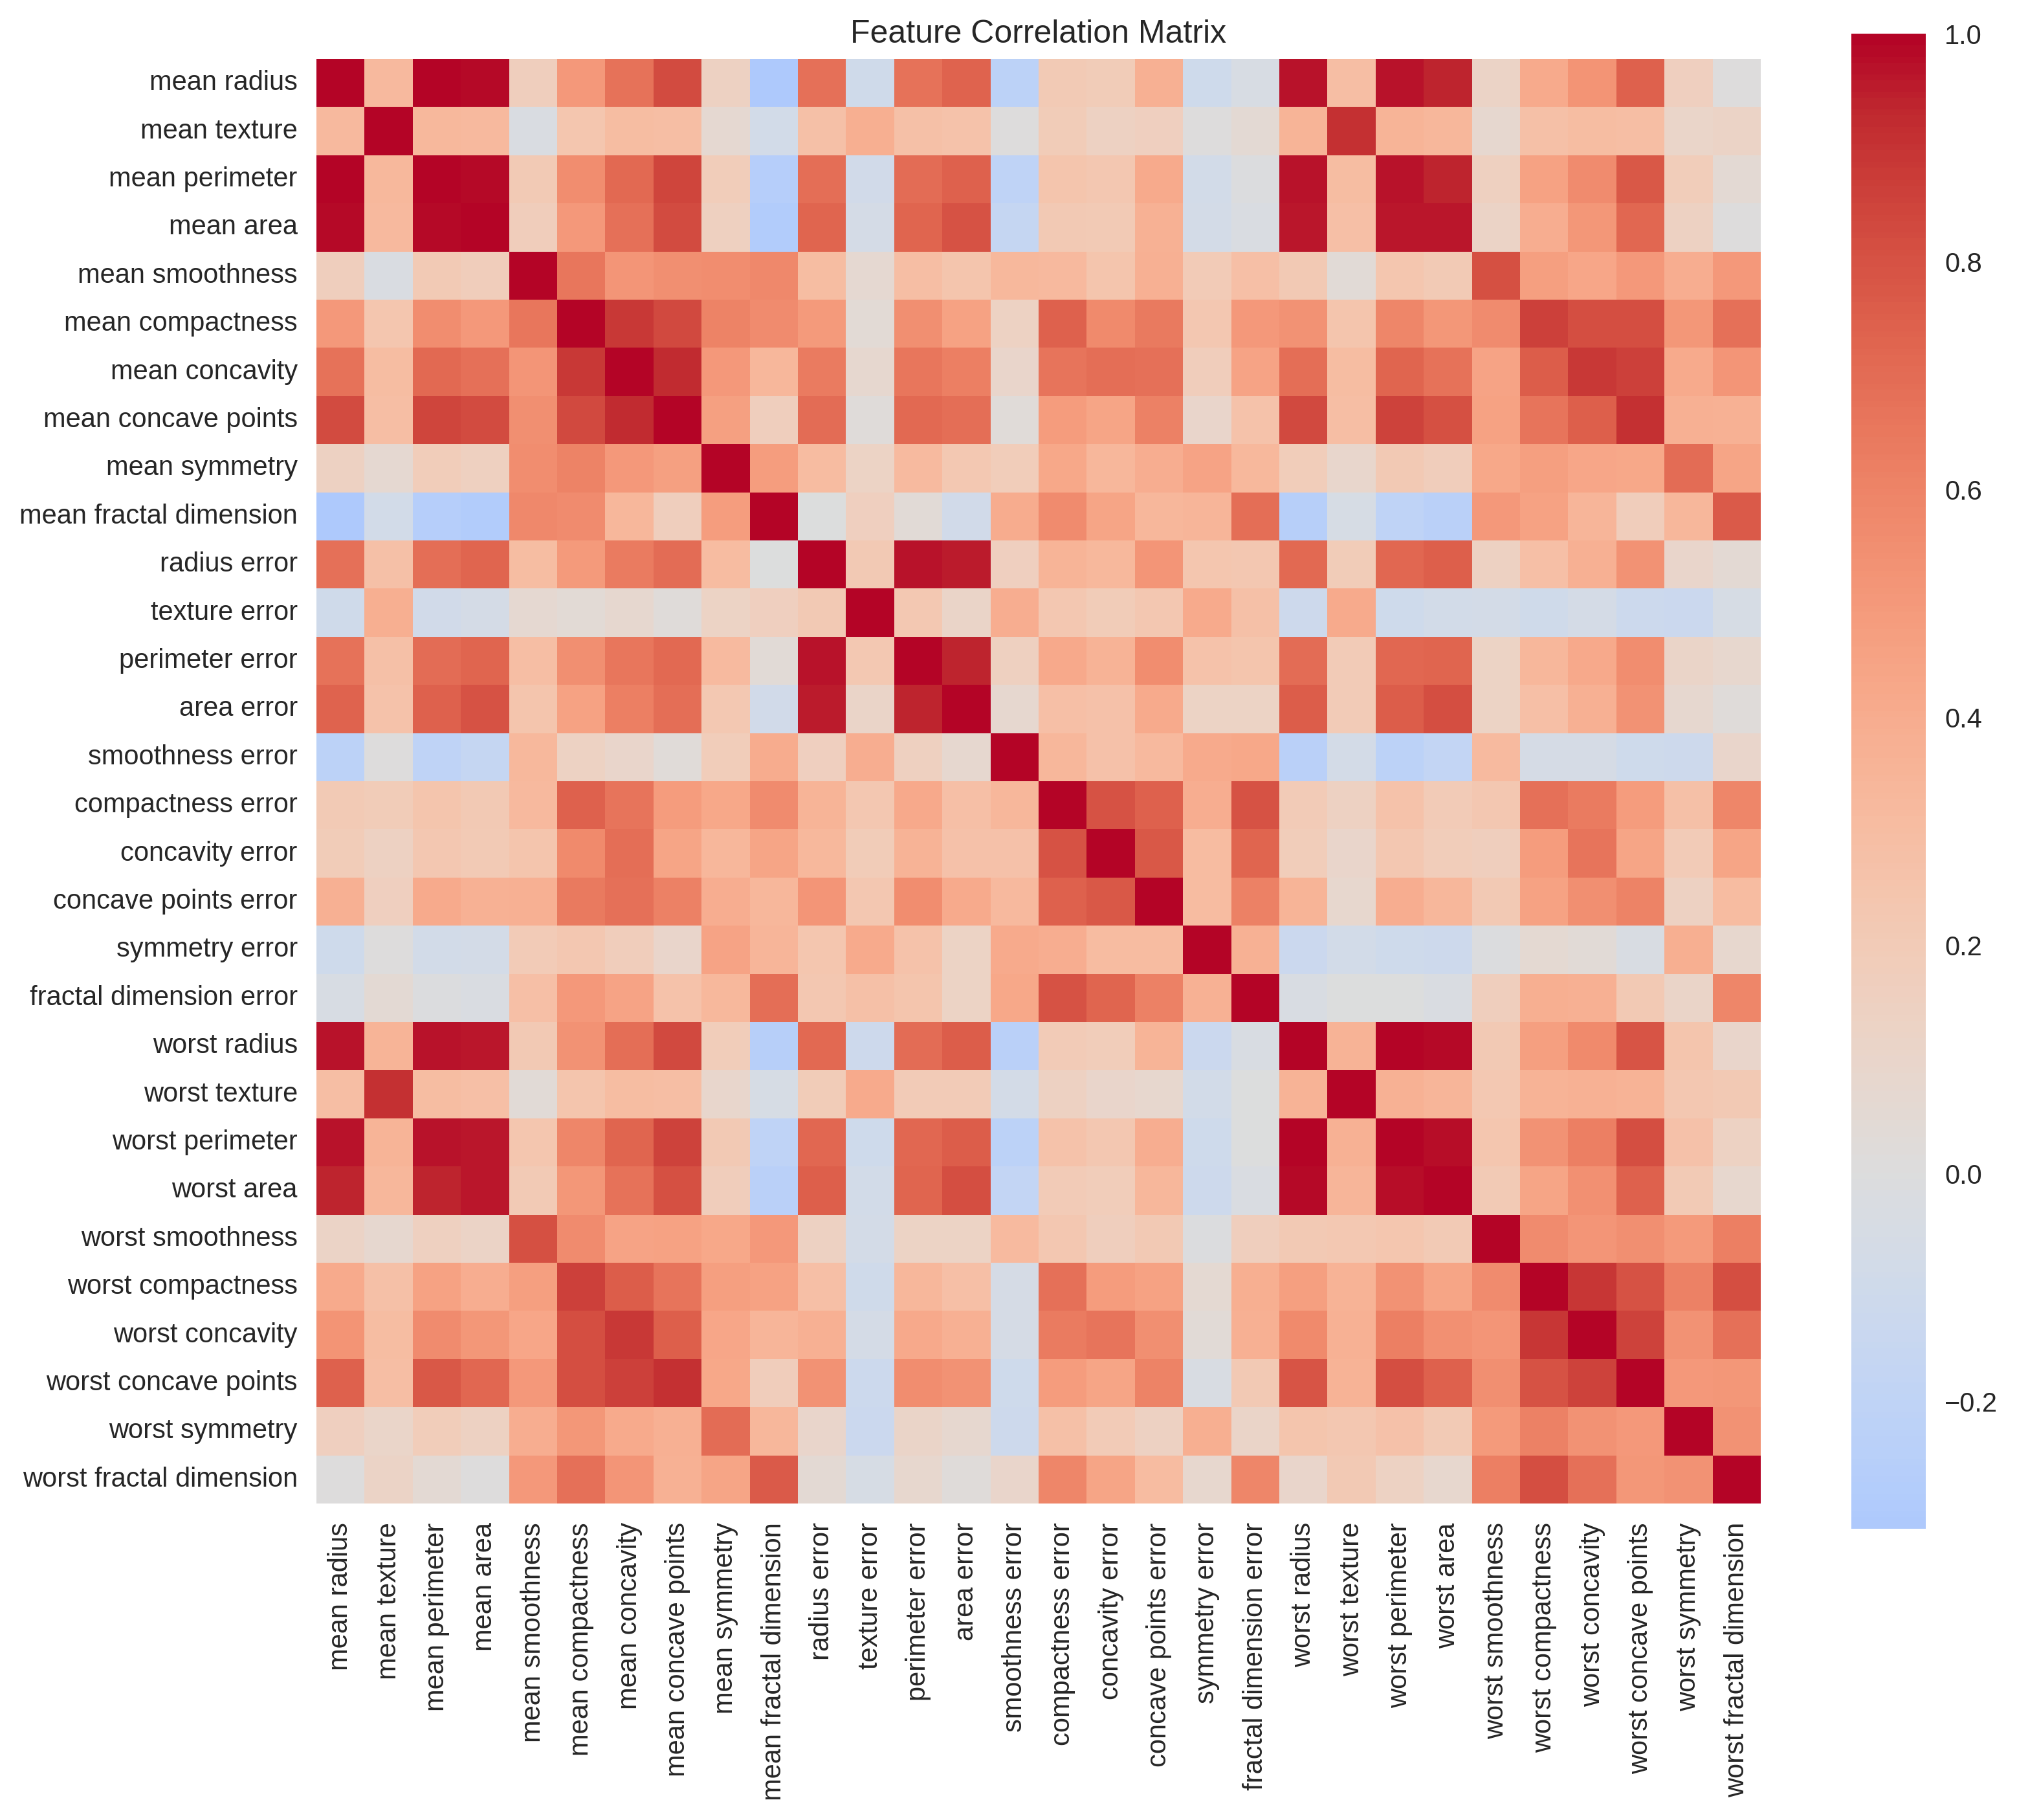
\includegraphics[width=0.75\textwidth]{../code/ch1_preprocessing/plots/breast_cancer_correlation_heatmap.png}
    \caption{Ma trận tương quan Breast Cancer: Xác định các cụm đặc trưng có tính đa cộng tuyến cao, hỗ trợ bước lựa chọn đặc trưng sau này.}
\end{figure}

\textbf{Giải thích chi tiết:} Heatmap cho thấy các cụm đặc trưng có tương quan cao: mean radius, mean perimeter, mean area (r=0.99) tạo thành một cụm; các đặc trưng texture, compactness, concavity cũng tương quan mạnh. Đây là hiện tượng đa cộng tuyến (multicollinearity), có thể gây vấn đề cho Linear Regression (giảm tính ổn định của coefficients). Feature selection hoặc PCA có thể cần thiết để giảm chiều dữ liệu.

\begin{figure}[H]
    \centering
    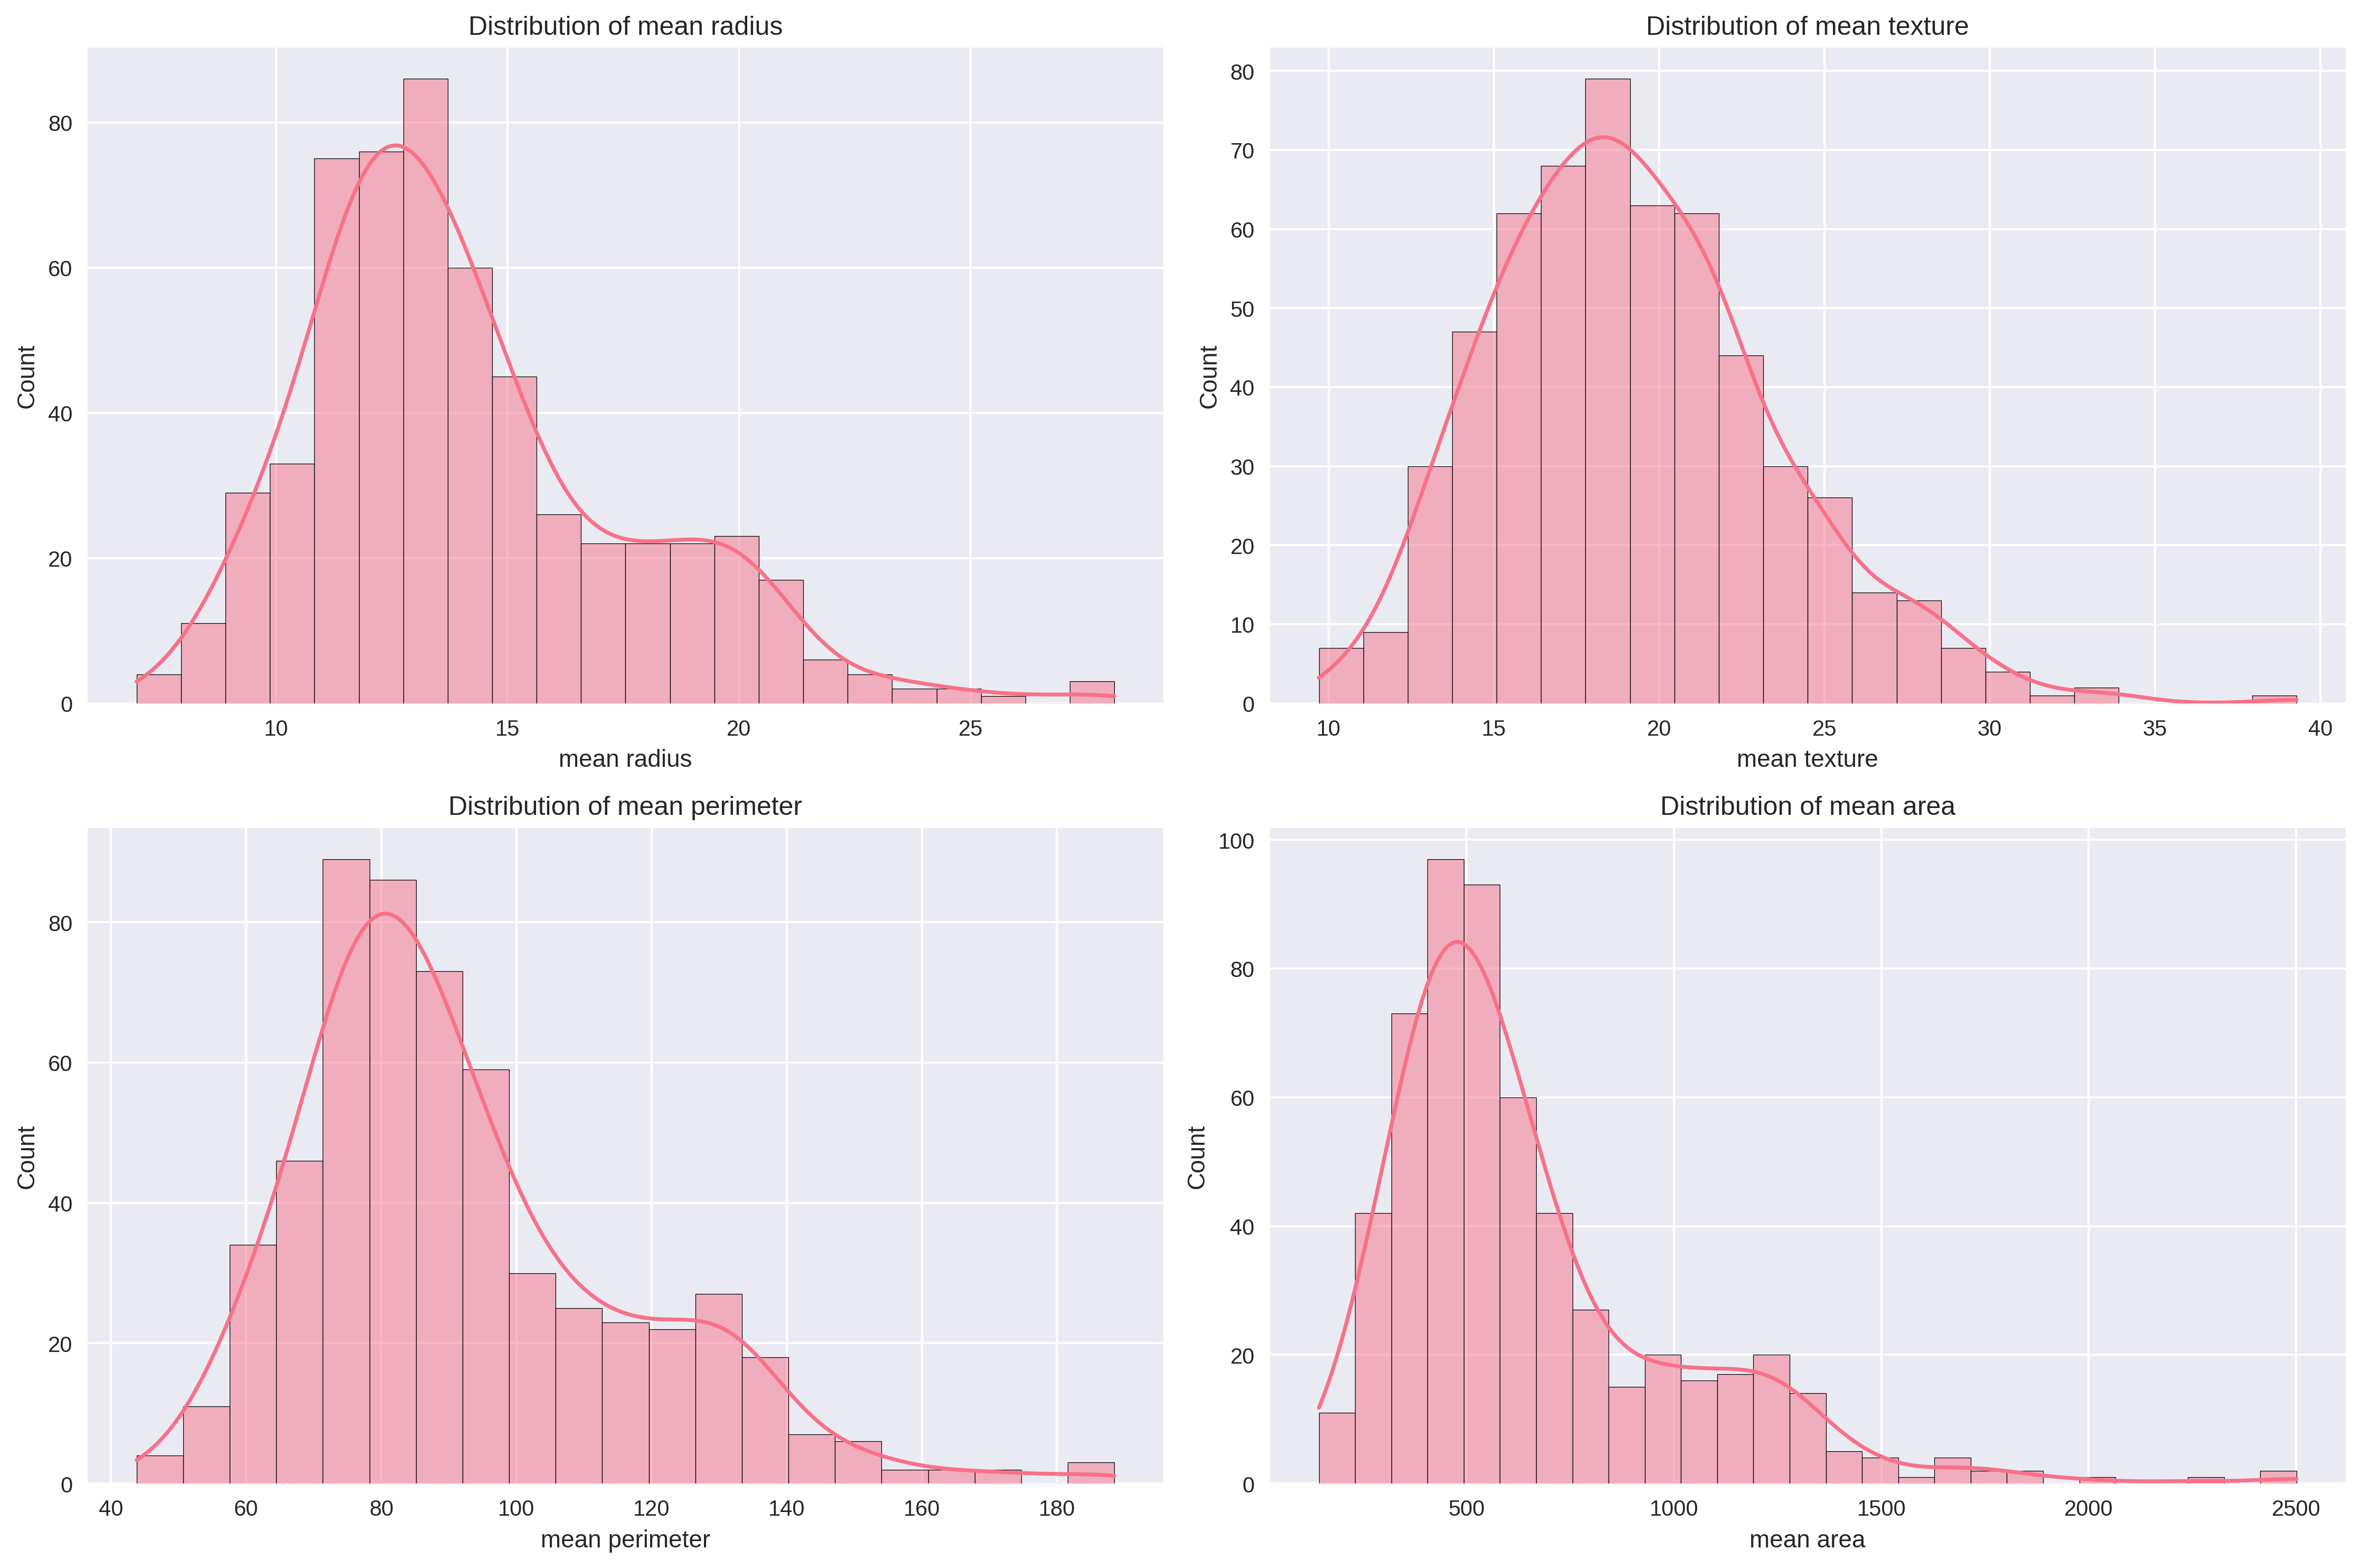
\includegraphics[width=0.75\textwidth]{../code/ch1_preprocessing/plots/breast_cancer_feature_distributions.png}
    \caption{Phân phối các đặc trưng: So sánh phân phối của các thuộc tính quan trọng giữa hai nhóm Lành tính và Ác tính.}
\end{figure}

\textbf{Giải thích chi tiết:} Biểu đồ KDE chồng lên nhau cho thấy sự khác biệt về phân phối giữa malignant (đỏ) và benign (xanh). Ví dụ, malignant có mean radius cao hơn rõ rệt. Điều này chứng minh discriminative power của các đặc trưng, hỗ trợ cho việc sử dụng chúng trong mô hình phân loại. Việc phân tích phân phối theo class giúp hiểu rõ pattern của dữ liệu, từ đó thiết kế feature engineering phù hợp.

\begin{figure}[H]
    \centering
    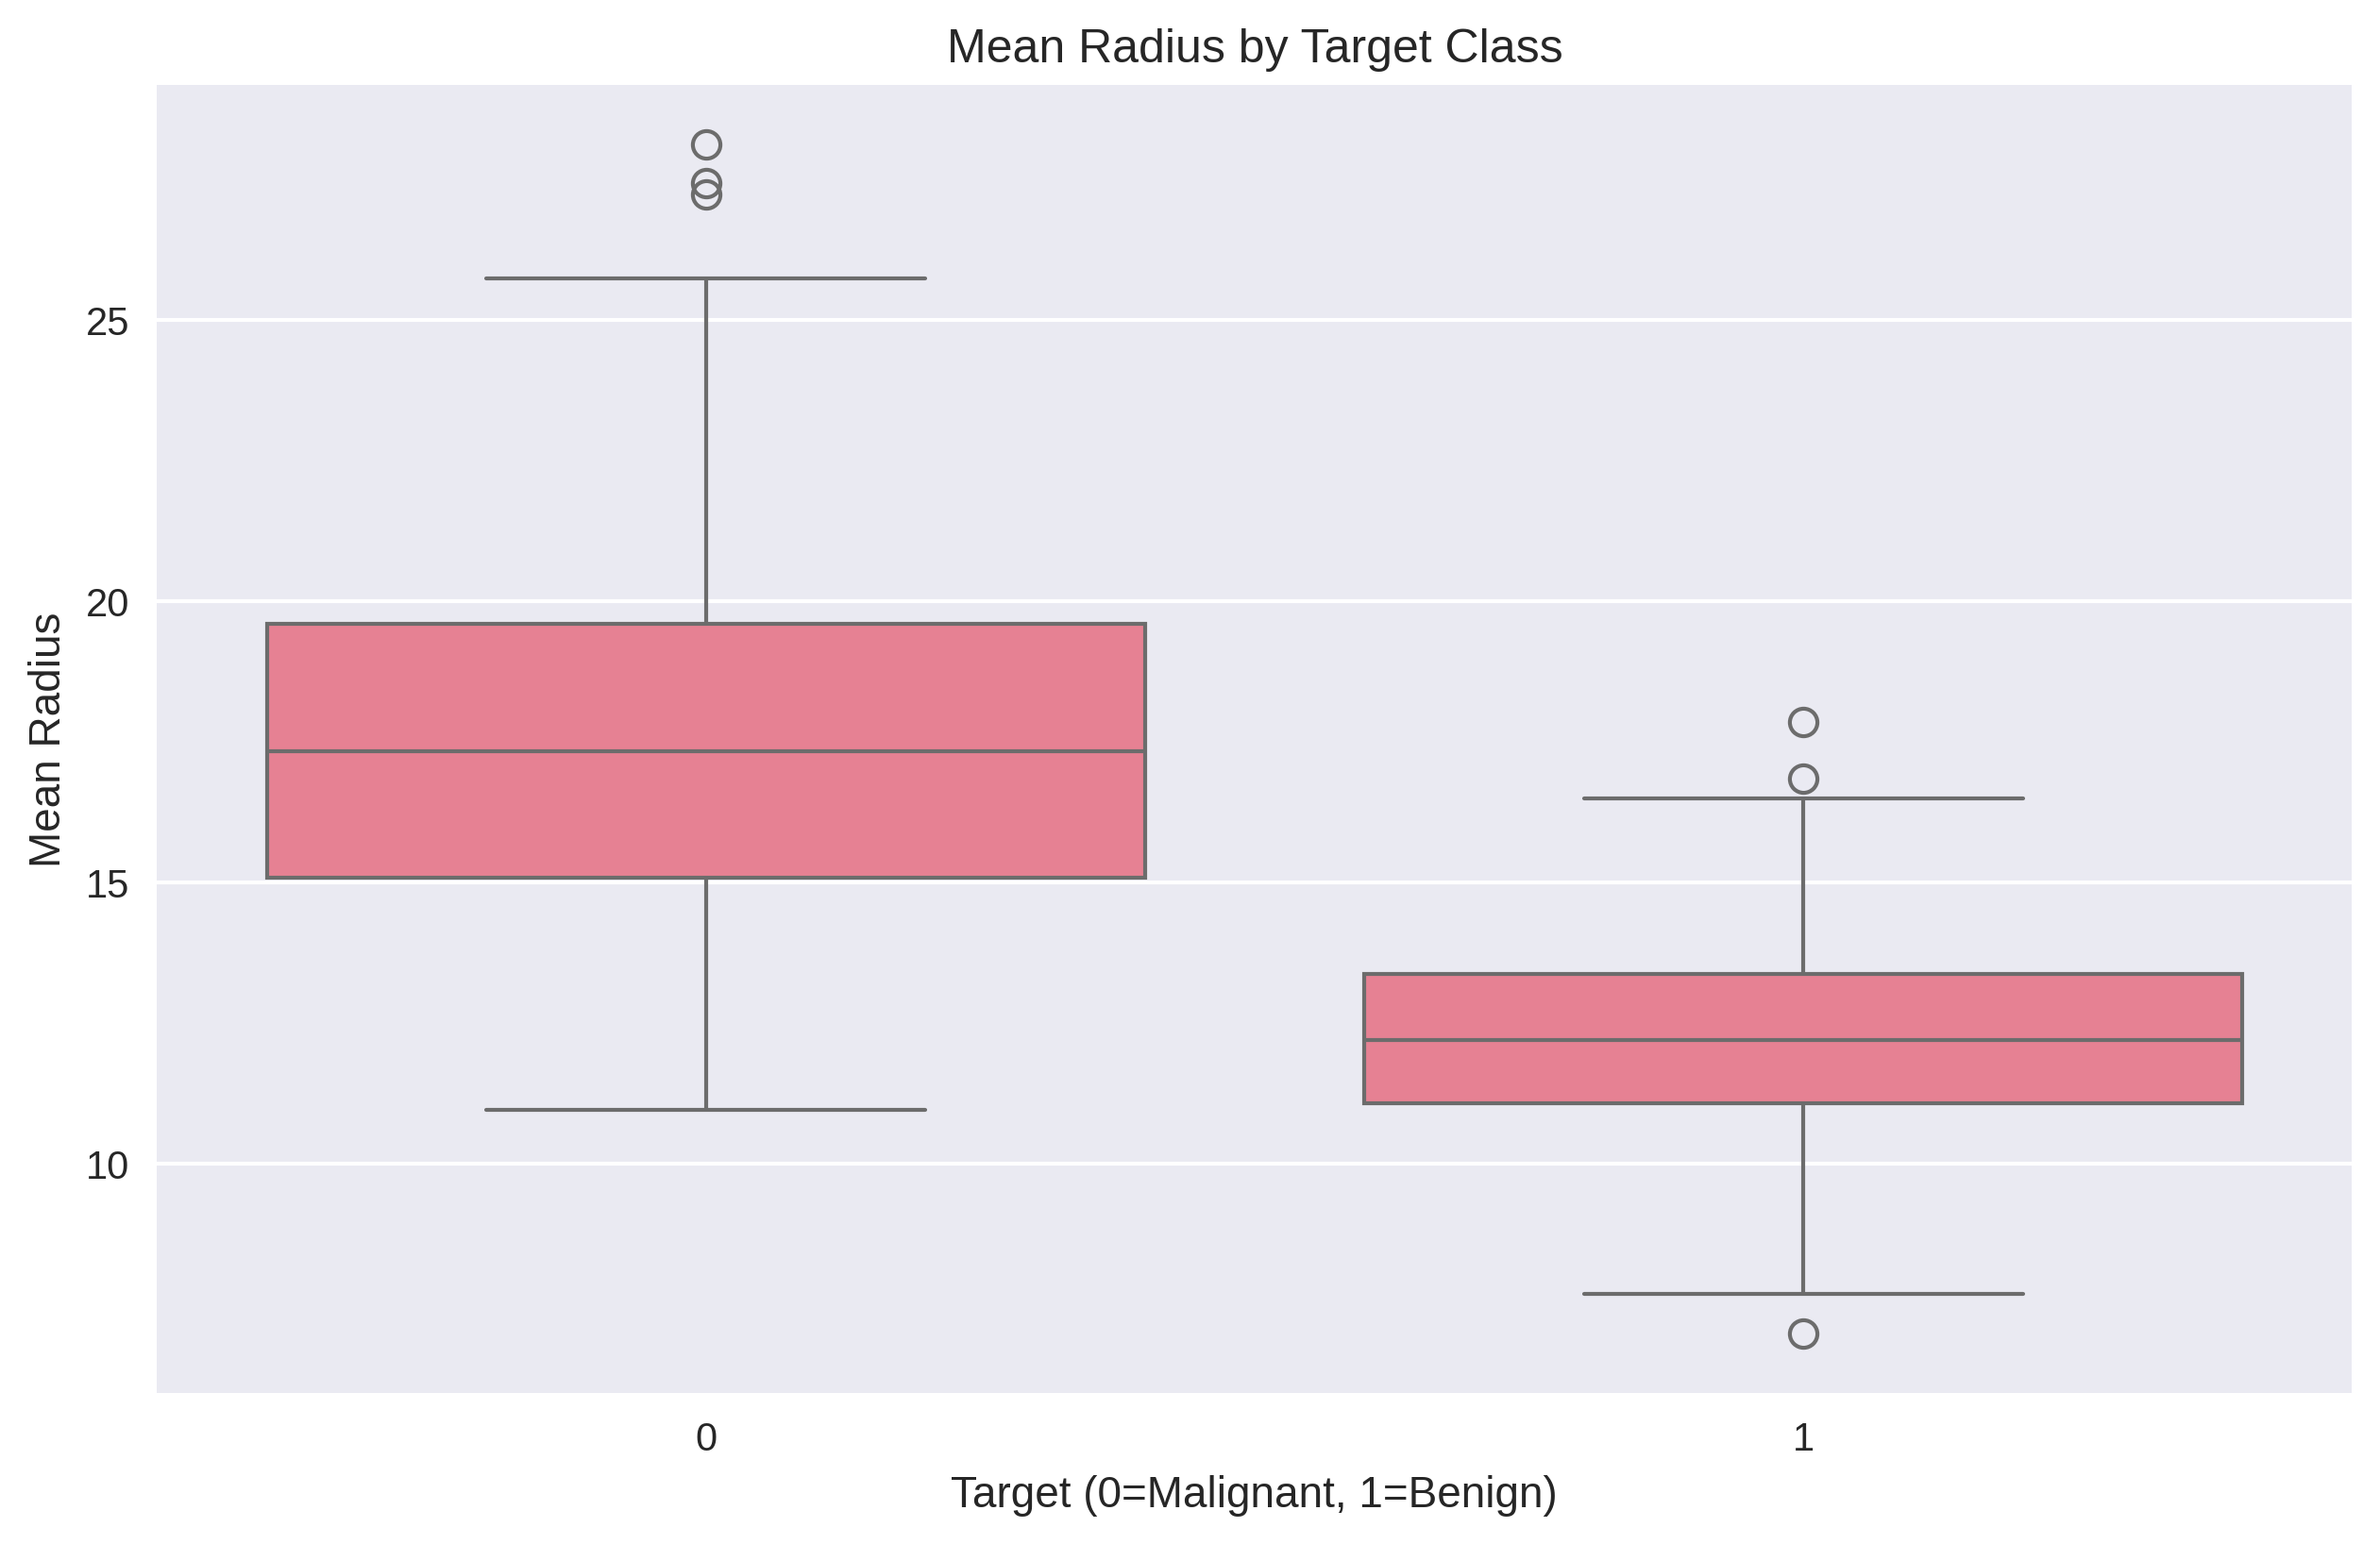
\includegraphics[width=0.75\textwidth]{../code/ch1_preprocessing/plots/breast_cancer_target_vs_radius.png}
    \caption{Mối quan hệ giữa Radius và nhãn mục tiêu: Trực quan hóa khả năng phân tách của đặc trưng 'mean radius'.}
\end{figure}

\textbf{Giải thích chi tiết:} Scatter plot với màu sắc theo class cho thấy mean radius là đặc trưng discriminative tốt: malignant (màu cam) có radius cao hơn benign (màu xanh). Tuy có overlap, nhưng rõ ràng có separation. Điều này giải thích tại sao radius thường được sử dụng trong chẩn đoán ung bướu - tế bào ác tính thường lớn hơn và phát triển nhanh hơn. Biểu đồ này minh họa trực quan lý thuyết về feature importance trong machine learning.

Tiến hành chuẩn hóa dữ liệu bằng các phương pháp khác nhau để tìm ra kỹ thuật tối ưu.

\begin{figure}[H]
    \centering
    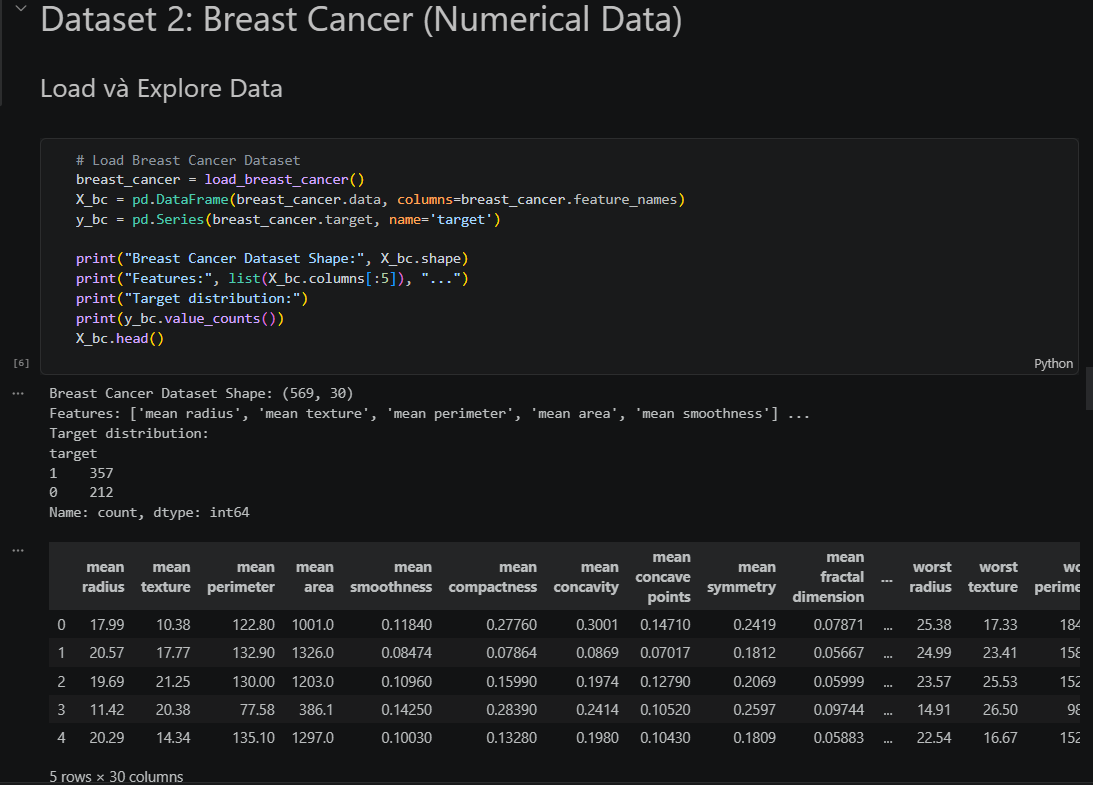
\includegraphics[width=0.9\textwidth]{../code/ch1_preprocessing/images/8.png}
    \caption{Triển khai các kỹ thuật Scaling: StandardScaler (Z-score) và MinMaxScaler để đưa dữ liệu về cùng một miền giá trị.}
\end{figure}

\textbf{So sánh lý thuyết:} Việc sử dụng \textbf{StandardScaler} (Z-score) giúp đưa dữ liệu về phân phối chuẩn ($\mu=0, \sigma=1$). Điều này đặc biệt quan trọng cho các thuật toán như SVM hay Logistic Regression vốn nhạy cảm với thang đo của dữ liệu đầu vào.

\begin{figure}[H]
    \centering
    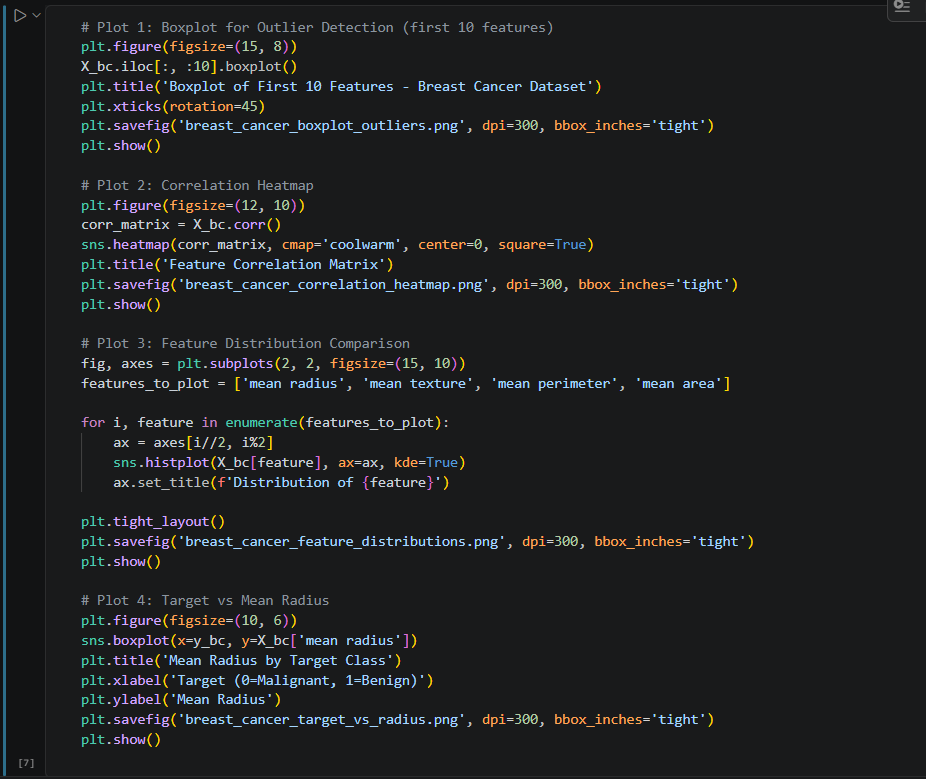
\includegraphics[width=0.9\textwidth]{../code/ch1_preprocessing/images/9.png}
    \caption{So sánh tác động của Scaling: Phân tích kết quả dự báo trước và sau khi áp chuẩn hóa Z-score.}
\end{figure}

Để kết thúc quy trình, chúng ta tổ chức lưu trữ các kết quả phân tích.

\begin{figure}[H]
    \centering
    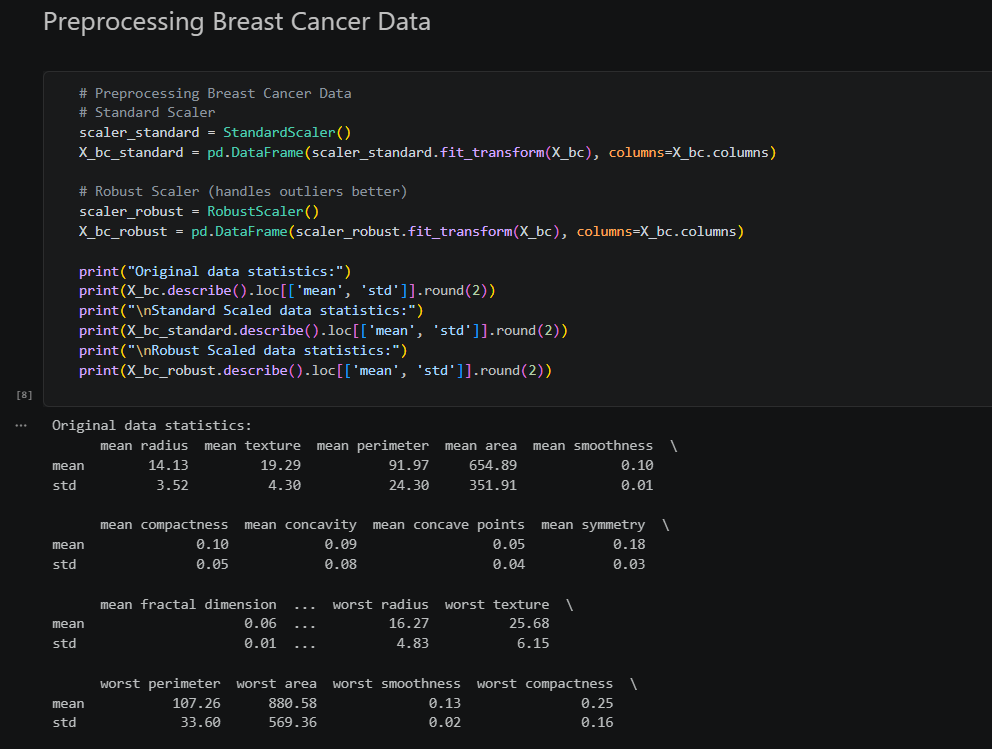
\includegraphics[width=0.9\textwidth]{../code/ch1_preprocessing/images/10.png}
    \caption{Quản lý hệ thống: Mã nguồn tự động tạo cấu trúc thư mục để lưu trữ các biểu đồ đầu ra chuyên nghiệp.}
\end{figure}

\begin{figure}[H]
    \centering
    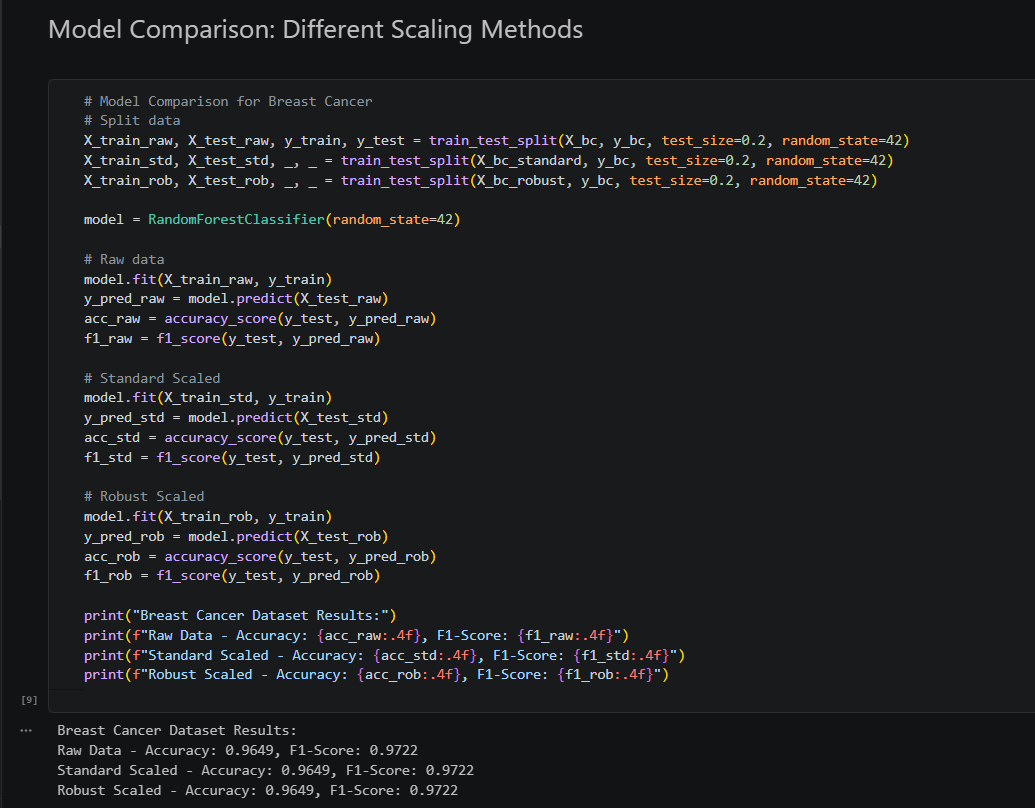
\includegraphics[width=0.9\textwidth]{../code/ch1_preprocessing/images/11.png}
    \caption{Hoàn tất quy trình: Thông báo kết thúc chuỗi xử lý và sẵn sàng dữ liệu cho giai đoạn Modeling.}
\end{figure}

\subsection{Kết luận Chương 1}
Trong chương này, chúng ta đã đi qua quy trình tiền xử lý dữ liệu đầy đủ từ EDA, xử lý dữ liệu khuyết, mã hóa đến chuẩn hóa. Qua hai bài toán thực tế Titanic và Breast Cancer, chúng ta thấy rằng mỗi loại dữ liệu đòi hỏi một chiến lược tiền xử lý riêng biệt.

Việc chuẩn bị dữ liệu kỹ lưỡng không chỉ giúp tăng độ chính xác của mô hình mà còn giúp giảm thiểu thời gian huấn luyện và tăng tính giải thích được cho các kết quả nghiên cứu.
